% !TeX program = lualatex
% !TeX spellcheck = en_US
\documentclass[
	paper=a4,
	open=right, % Chapters start on right pages
	twoside=true,
	fontsize=11pt,
	parskip=full % Space between paragraphs
]{scrreprt}

% % % Polyglossia % % %
\usepackage{polyglossia}
\setmainlanguage[variant=american]{english}

% % % csquotes % % %
\usepackage{csquotes}

% % % BibLaTeX % % %
\usepackage[
	%abbreviate=false, % Don't abbreviate standard bibliography terms
	backend=biber, % Bibliography engine
	citestyle=numeric-comp, % Style for citations
	bibstyle=numeric, % Style for bibliography
	date=terse, % Shorter dates
	ibidtracker=false, idemtracker=false, opcittracker=false, citetracker=false, % Don't abbreviate when same citation twice in a row
	doi=false, % Don't print the following fields in the bibliography, unless required by the entry type
	isbn=false,
	url=false,
	giveninits=true, % Render first and middle names as initials
	uniquename=init, % Prevent using initials for authors
	maxcitenames=2, % Maximum number of authors to use in citations
	maxbibnames=99 % Print all authors in bibliography
]{biblatex}

\bibliography{quellen}

\setlength{\bibitemsep}{.7\baselineskip} % Empty lines between literature sources

\renewcommand{\labelnamepunct}{\addcolon\addspace} % Colon between author and title in bibliography

% General settings
\setcounter{tocdepth}{2} % Show chapters, sections, and subsection in the table of contents
\interfootnotelinepenalty=10000 % Prevent breaking of footnotes across pages

% % % ToCloft % % %
\usepackage[titles]{tocloft}
\setlength{\cftbeforechapskip}{0.5\baselineskip}

% % % Import % % %
%\usepackage{import}

% % % Bookmark % % %
\usepackage[open,openlevel=1]{bookmark}

% % % VarioRef % % %
%\usepackage{varioref}
\newcommand\vref{\ref} % disabling varioref because it causes unstable typesetting

% % % GraphicX % % %
\usepackage{graphicx}
\graphicspath{{bilder/}{grafiken/}{screenshots/}{gnuplot/plots/}}

% % % SVG % % %
% Since we use lualatex, some pdftex commands need to be imported first
%\usepackage{pdftexcmds}
%\makeatletter
%\let\pdfstrcmp\pdf@strcmp
%\let\pdffilemoddate\pdf@filemoddate
%\makeatother

%\usepackage[svgpath=grafiken/]{svg}

% % % TabularY % % %
\usepackage{tabulary}
\usepackage{multirow}
\usepackage{hhline}

% % % Glossaries % % %
\usepackage[toc,nonumberlist]{glossaries}
% TODO: use acronym entries instead of glossary
\newglossaryentry{mpsoc}{
    name = {MPSoC},
    description = {Multi-Processor System-on-Chip},
    plural = {MPSoCs}
}
\newglossaryentry{noc}{
    name = {NoC},
    description = {Network-on-Chip},
    plural = {NoCs}
}
\newglossaryentry{pe}{
    name = {PE},
    description = {Processing Element},
    plural = {PEs}
}
\newglossaryentry{ni}{
    name = {NI},
    description = {Network Interface},
    plural = {NIs}
}
\newglossaryentry{aes}{
    name = {AES},
    description = {Advanced Encryption Standard}
}
\newglossaryentry{ip}{
    name = {IP},
    description = {Intellectual Property},
    plural = {IPs}
}
\newglossaryentry{gals}{
    name = {GALS},
    description = {Globally Asynchronous, Locally Synchronous}
}
\newglossaryentry{dos}{
    name = {DoS},
    description = {Denial of Service}
}
\newglossaryentry{gev}{
    name = {GEV},
    description = {Global Encoding Vector},
    plural = {GEVs}
}
\newglossaryentry{amd}{
    name = {AMD},
    description = {Algebraic Manipulation Detection}
}
\newglossaryentry{crc}{
    name = {CRC},
    description = {Cyclic Redundancy Check}
}
\newglossaryentry{arq}{
    name = {ARQ},
    description = {Automatic Repeat reQuest},
    plural = {ARQs}
}
\newglossaryentry{tcp}{
    name = {TCP},
    description = {Transmission Control Protocol}
}
\newglossaryentry{mac}{
    name = {MAC},
    description = {Message Authentication Code},
    plural = {MACs}
}
\newglossaryentry{romm}{
    name = {ROMM},
    description = {Randomized, Oblivious, Multi-phase, Minimal}
}
\newglossaryentry{dsr}{
    name = {DSR},
    description = {Dynamic Smart Random}
}
\newglossaryentry{fifo}{
    name = {FIFO},
    description = {First In, First Out}
}
\newglossaryentry{asic}{
    name = {ASIC},
    description = {Application-Specific Integrated Circuit},
    plural = {ASICs}
}
\newglossaryentry{fpga}{
    name = {FPGA},
    description = {Field-Programmable Gate Array},
    plural = {FPGAs}
}

\makeglossaries

% % % EnumItem % % %
\usepackage{enumitem}
\setitemize{itemsep=-.5\parskip, topsep=-.5\baselineskip}
\setenumerate{itemsep=-.5\parskip, topsep=-.5\baselineskip}

% % % Titling % % %
\usepackage{titling}

% % % Caption % % %
\usepackage[font={small,it}]{caption}

% % % math packages % % %
\usepackage{mathtools}
\usepackage{amsmath}
\usepackage{amssymb}

% % % ChangeCounter % % %
%\usepackage{chngcntr}
%\counterwithout{footnote}{chapter} % Global footnote indices

% % % ChangePage % % %
\usepackage{changepage}

% % % EPStoPDF % % %
\usepackage{epstopdf}

% % % PDFpages % % %
\usepackage{pdfpages}

% % % Color % % %
\usepackage{color}

% % % SIunitX % % %
\usepackage[group-separator={,}]{siunitx}

% % % Rahmendaten % % %
\author{Julian Harttung}
\title{Secure and Efficient Communication for Network-on-Chip under the Consideration of Multiple Paths}
\newcommand{\thesubtitle}{Diploma Thesis}
\newcommand{\theuniversity}{Dresden University of Technology}
\newcommand{\thefaculty}{Faculty of Computer Science}
\newcommand{\theinstitute}{Institute of Systems Architecture}
\newcommand{\thechair}{Chair of Privacy and Data Security}
% % % Rahmendaten Ende % % %

% Hilfsmakros
\newcommand{\omnet}{OMNeT++}

% Platzhalter für Evaluationsparameter
\newcommand{\pProtVar}{\ensuremath{v}} % Protocol variant
\newcommand{\pNCMode}{\ensuremath{n}} % Network coding mode
\newcommand{\pEncMods}{\ensuremath{e}} % Number of encryption modules
\newcommand{\pAuthMods}{\ensuremath{a}} % Number of authentication modules
\newcommand{\pRQSize}{\ensuremath{q}} % Queue size limit for router←→router input queues
\newcommand{\pARQLimit}{\ensuremath{l}} % ARQ Limit
\newcommand{\pARQTimeout}{\ensuremath{t_1}} % ARQ flit inter-arrival timeout
\newcommand{\pRStrat}{\ensuremath{r}} % Routing strategy
\newcommand{\pAttackerSet}{\ensuremath{s}} % Which set of 8 malicious routers is used
\newcommand{\pAttackProb}{\ensuremath{p}} % Probability of an attack

\begin{document}
    \frenchspacing % Disable double spaces between sentences
	\begin{titlepage}
		
\includegraphics[width=0.25\textwidth]{TU_Dresden_Logo_blau_HKS41}
		\hfill
		
\includegraphics[width=0.23\textwidth]{HAEC_Logo_cmyk}
		\vspace{1.5\baselineskip}
		
		\begin{center}
			\textsc{\theuniversity \\
					\thefaculty \\
					\theinstitute \\
					\thechair}
			\vspace{2.5\baselineskip}
		
			\Huge{\thetitle}
			\vspace{.5\baselineskip}
			
			\LARGE{\thesubtitle}
		\end{center}
		
		\vfill
		
		\begin{tabular}{ll}
			Author:               & \theauthor \\
			Course of Studies:    & Diplom-Informatik (PO 2010)\\
			Matriculation Number: & 3753196 \\
			Supervisors:          & Dr.-Ing. Elke Franz and Dipl.-Inf. Paul Walther \\
			Professor:            & Prof. Dr. Thorsten Strufe \\
			\multicolumn{2}{l}{ } \\
			\multicolumn{2}{l}{ } \\
			\multicolumn{2}{l}{ } \\
			\multicolumn{2}{l}{Dresden, June 28, 2018}
		\end{tabular}
	\end{titlepage}
	
	
	\pagenumbering{roman}
	
    % Task page
    
\includepdf[pages={-}]{aufgabe.pdf}
	
    \chapter*{Selbstständigkeitserklärung}
    Hiermit erkläre ich, dass ich die von mir am heutigen Tag dem Prüfungsausschuss der Fakultät Informatik eingereichte Arbeit zum Thema:
    \begin{adjustwidth}{0.15\textwidth}{0.15\textwidth}
        \begin{center}
            \textit{\thetitle}
        \end{center}
    \end{adjustwidth}

    vollkommen selbstständig verfasst und keine anderen als die angegebenen Quellen und Hilfsmittel benutzt sowie Zitate kenntlich gemacht habe.

    \vspace{0.5\baselineskip}
    Dresden, 28.\ Juni 2018 \\

    \vspace{1.5\baselineskip}
    \theauthor

	\chapter*{Acknowledgement}
    In addition to my supervisors, I would like to thank M.Sc. EE Sadia Moriam from the TU Dresden Vodafone Chair Mobile Communications Systems for
    her invaluable counsel throughout the process of creating this diploma thesis.
	
	\tableofcontents
	
	\addtocontents{lot}{\protect\vspace{-1.4\baselineskip}}
	\addtocontents{lof}{\protect\vspace{-1.4\baselineskip}}
	
	\listoftables
	\vspace{-2.6\baselineskip}
	\begingroup
	\let\clearpage\relax
	\listoffigures
	\endgroup
	
	
	\chapter{Introduction}\label{ch:introduction}
	\pagenumbering{arabic}
    The computing power of integrated circuits has been growing steadily since the dawn of the digital age. In the 20th century, this was mainly achieved
by increasing their clock frequencies to allow for faster executions of the hardware instructions. However, with the beginning of the new millenium,
clock speeds ceased to experience substantial growth rates, mainly due to physical limitations \cite{intelfrequency}. Thus, the focus of circuit
designers shifted to other avenues of performance gains. With Moore's Law still proving to be accurate \cite{mack11mooreslaw}, the number of
transistors fitting onto a single die continues to increase to this day, stimulating the trend towards highly parallelized systems where multiple
processing cores operate side by side \cite[6]{kumar08parallel}. Hence, today's performance gains often stem from a higher level of parallelism
instead of speed increases within single cores.

As the number of processing cores continues to rise, the importance of having an efficient interconnection architecture capable of handling such
highly parallelized systems grows as well. Traditional interconnection architectures employ a global bus that all cores are attached to. However,
buses quickly became a bottleneck for the overall performance \cite[6]{tatas16designingnocs} as their bandwidth is shared by all connected cores. To confront this
scaling problem, novel interconnection approaches were developed, and thus the \textit{Network-on-Chip (\gls{noc})} paradigm was devised
\cites{kumar02networkonchip}{benini02nocparadigm}. It is explained in detail in Section \ref{sec:networkonchipfun}.

\Glspl{noc} scale significantly better with the number of cores and aim to overcome the drawbacks of traditional buses, which is also elaborated in
Section \ref{sec:networkonchipfun}. However, as the popularity of \glspl{noc} increases, so does the interest of adversaries to compromise systems
that implement them as their communication backbone. Particularly due to the trend of chip manufacturers integrating a growing amount of third party components, the
threat of the hardware itself being compromised becomes increasingly relevant \cites{ancajas14fortnocs}{sethumadhavan15trustworthyhardware}.

In order to counteract such threats, it is desirable to embed security considerations directly into the design phase of the circuits (cf. Section
\ref{sec:nocsecurity}). In recent research, numerous approaches to integrate such security measures have been pursued\footnote{For an elaborate
discourse on related research, see Chapter \ref{ch:relatedwork}.}. At the TU Dresden Chair of Privacy and Data Security, a method to protect the
communications between the cores against adversaries residing in the networking hardware was explored
\cites{moriam15manycorenc}{moriam18activeattackers}. In their approach, network coding was combined with authentication, yielding a significant
increase of their system's resilience to active attackers.

This thesis sets out to expand and improve this approach. Aiming to enhance both performance and security, their scheme is augmented through the
addition of encryption and multipath routing, amongst others.

For the TU Dresden, \gls{noc}-related research is of particular importance. In a large-scale, interdisciplinary research project called \textit{Highly
Adaptive and Energy-efficient Computing (\gls{haec})}, a novel approach for massively parallel computing is pursued \cite{matthiesen17haec}. In this
project, a new 3D processor architecture is designed that encompasses numerous compute nodes, each containing \enquote{thousands of […] cores […] to
offer massive intra-node parallelism} \cite[1]{matthiesen17haec}. Hence, an efficient and secure intra-node interconnection system is crucial to
ensure flawless operation of the system. A visualization of their design is given in Figure \vref{fig:haecbox}.

\begin{figure}
    \centering
    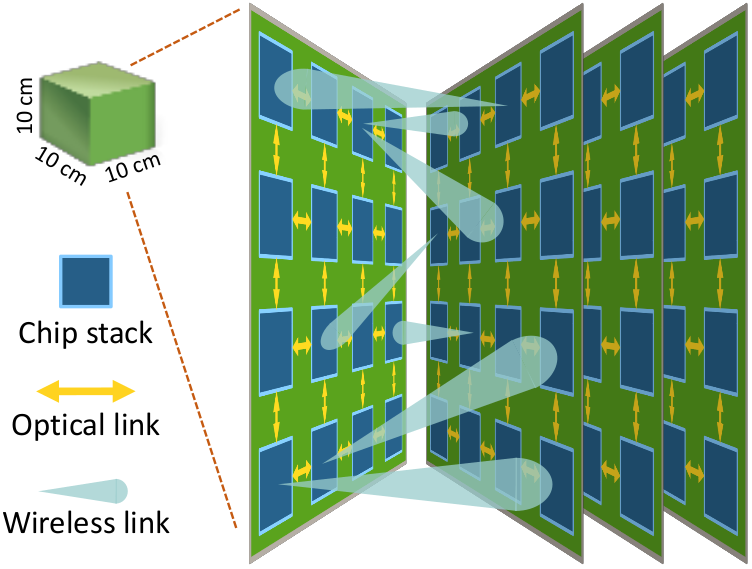
\includegraphics[width=0.4\textwidth]{haecbox}
    \caption[Processor architecture in the HAEC project]{Processor architecture employed in the \gls{haec} project. Numerous chip stacks are organized
    in compute boards and employ optical and wireless links for their interconnection. Each chip stack is a compute node consisting of of multiple
    cores arranged as a 3D mesh, which are interconnected by a wired \gls{noc}. The illustration is taken from the \gls{haec} presentation paper
    \cite[1]{matthiesen17haec}.}
    \label{fig:haecbox}
\end{figure}

The main contributions of this thesis are the conceptualization, implementation, and evaluation of a new approach for secure and efficient
communications in a \gls{noc} that is based upon the foundational work of \citeauthor{moriam18activeattackers}
\cites{moriam15manycorenc}{moriam18activeattackers}. This encompasses the design of an improved communication protocol in multiple variants and its
extensive evaluation through software simulation.

The thesis begins with an explanation of key terms and concepts that are essential for the comprehension of the remainder of this work (Chapter
\ref{ch:fundamentals}). Afterwards, a discourse on related research in the field of \glspl{noc} and their security is provided (Chapter
\ref{ch:relatedwork}). Subsequently, Chapter \ref{ch:overview} gives an overview of the methodologies and courses of action that were employed in this
thesis, followed by an exhaustive and detailed description of the designed communication protocol in Chapter \ref{ch:protocol}. Then, the
implementation of the simulator is presented (Chapter \ref{ch:implementation}) before evaluating the devised protocol (Chapter \ref{ch:evaluation}).
Finally, the thesis is concluded with a summary and an outlook on future work (Chapter \ref{ch:conclusion}).

    
    \chapter{Fundamentals}\label{ch:fundamentals}
    \section{Networks-On-Chip}\label{sec:networkonchipfun}
\textit{Network-on-Chip} (or \textit{\gls{noc}} for short) is a paradigm for interconnecting components on a chip. Typically employed on
\textit{Multi-Processor Systems-on-Chip (\glspl{mpsoc})} \cites(e.g.)(){ivanov05nocintroduction}{biswas15routerattack}{tatas16designingnocs}, they
provide the communication infrastructure for \textit{processing elements (\glspl{pe})} and possibly other \gls{ip} cores.

The topology of a \gls{noc} can vary. Researchers usually work with a 2D mesh topology
\cites(e.g.)(){frey17hardenednoc}{kumar02networkonchip}{fernandes16nocrouting}{boraten16packetsecurity}, which will also be used throughout this thesis.
In this case, each network node is connected to its four neighbors (excluding the boundary nodes).

A node typically consists of a processing element (often referred to as an \textit{\gls{ip} core} or just \textit{core}), a network interface,
and a router \cite{dally01routepacketsnotwires}. The router manages the connections to neighboring nodes while also allowing
the local processing element to communicate with the network through the network interface. An example of this architecture is given in Figure
\vref{fig:nocexample}.

Compared to traditional bus-based interconnect systems, \glspl{noc} can provide a lot of advantages, especially for many-core systems
\cite[5\psqq]{tatas16designingnocs}. One big advantage is scalability; because the cores do not share a global bus, \enquote{local performance is not
degraded} \cite[6]{tatas16designingnocs} as more components are added, and \enquote{aggregated bandwidth scales with the network size}
\cite[6]{tatas16designingnocs}.

In addition, the absence of global interconnection wires facilitates the use of different clock domains. This enables the implementation of the
\textit{globally asynchronous, locally synchronous (\gls{gals})} paradigm, which becomes increasingly important in chip design
\cites[3]{kumar02networkonchip}[2]{ivanov05nocintroduction}.

Furthermore, with the constantly increasing design complexity of modern chips \cite{mack11mooreslaw}, specialized on-chip
interconnections become infeasible to implement. Designing such a system \enquote{would take too much time and mapping of applications to dedicated
architectures would be impossible} \cite[1]{kumar02networkonchip}. In contrast, \glspl{noc} aims to be general purpose interconnect systems; they
\enquote{facilitate […] modularity by defining a standard interface} \cite[1]{dally01routepacketsnotwires}.

\begin{figure}
    \centering
    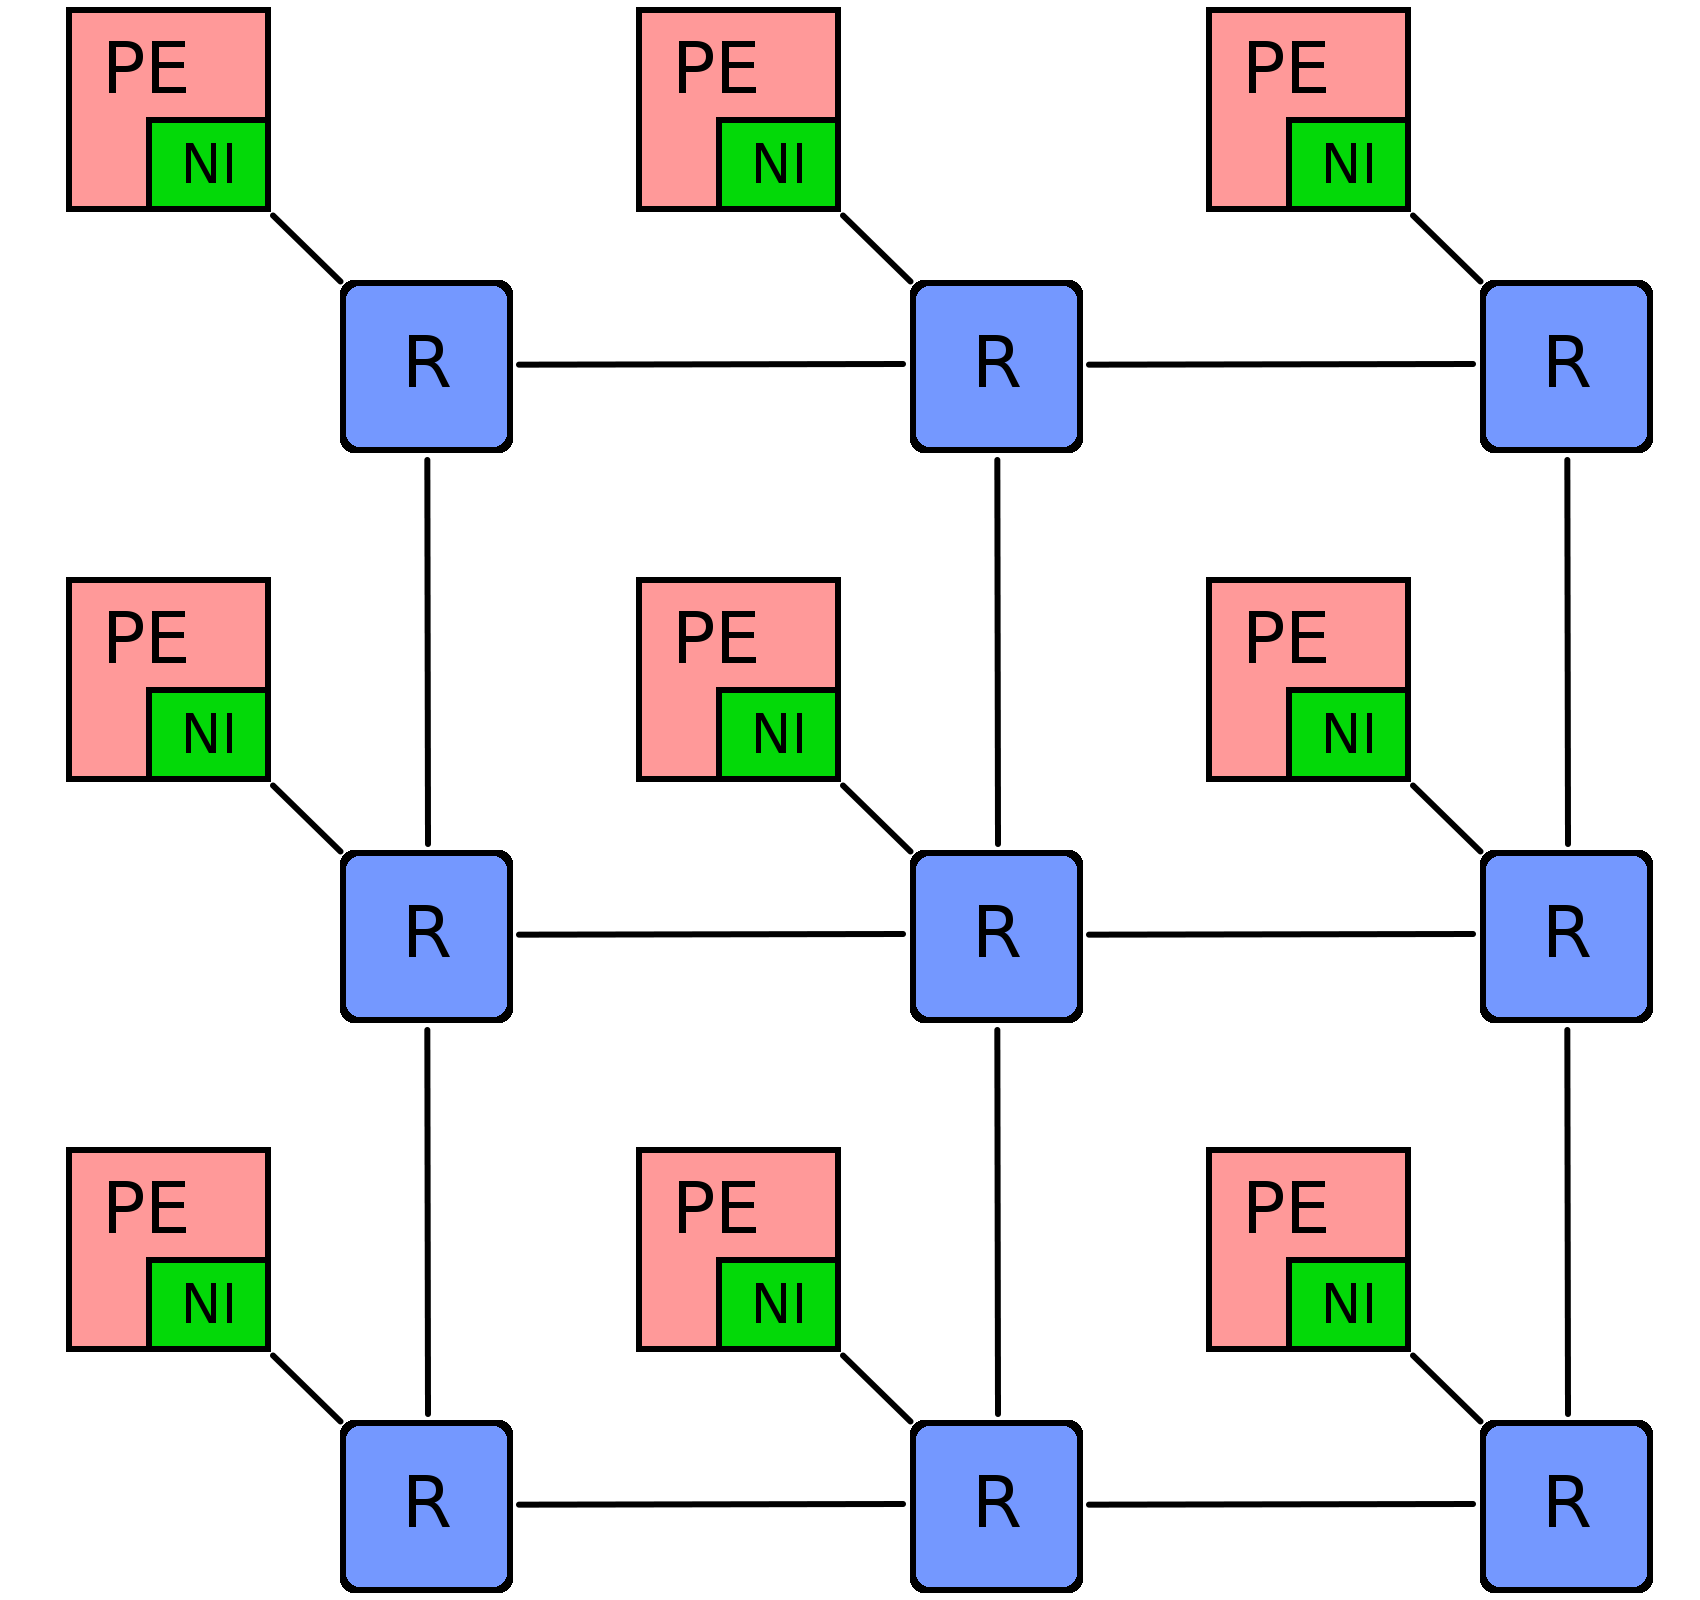
\includegraphics[width=0.6\textwidth]{noc_3x3_colored}
    \caption[Example of a 3x3 mesh NoC]{Example of a Network-on-Chip in a 2D mesh topology of size 3x3. The processing elements (red) contain a network interface
    (green) through which they are connected to a router (blue). The routers are interconnected as a 2D mesh.}
    \label{fig:nocexample}
\end{figure}

\section{Flits}\label{sec:flits}
Flits (short for \textit{flow control units}) are small pieces of data that are sent over a network. They are usually created by breaking a larger
packet down into parts that can be transmitted individually \cite[6]{flitslecturecmu}. Each flit must contain a set of header fields (such as source and
destination address, sequence number, or identifier) that are required for routing and handling \cite[2]{flitslectureutah}. In addition, it contains
a payload that carries the actual information to be transmitted.

In the context of \glspl{noc}, flits are often used as the standard unit of transmission \cite[51\psqq]{tatas16designingnocs}. Details on how flits
are used in this thesis can be found in (insert section/chapter vref).
% TODO: insert reference

\section{Hardware Trojans}\label{sec:hardwaretrojans}
% What are HTs, why can they get into other hardware, what are their properties
Hardware trojans are \enquote{malicious modifications of electronic hardware} \cite[1]{bhunia14hardwaretrojans} with the intent of disrupting normal
system behavior or extracting sensitive information. Because the integration of third party \gls{ip} has become increasingly popular due to circuit
complexity and cost efficiency \cites[1]{ancajas14fortnocs}[2]{bhunia14hardwaretrojans}, it is possible for adversaries to introduce hardware
trojans into larger systems, such as \glspl{mpsoc}.

In order to remain undetected, attackers aim to construct hardware trojans that are \enquote{stealthy in nature} \cite[1]{bhunia14hardwaretrojans}
and \enquote{evade […] detection through conventional postmanufacturing test} \cite[1]{bhunia14hardwaretrojans}. Hardware trojans are usually in a
dormant state until they are activated by a trigger signal to carry out their task \cites{bhunia14hardwaretrojans}{ancajas14fortnocs}. While the
trojan is inactive, communications through the \gls{noc} are unaffected and the system operates normally.

Attack types: information leak/eavesdropping, DoS (→ bandwidth depletion, deadlock, livelock)
% TODO: is this a fundamental? or write this when describing our attacker model?

\section{Network Coding}\label{sec:networkcodingfun}
Network coding is a technique for transmitting packets efficiently over a network. First described in 2000 by \citeauthor{ahlswede00networkflow}
\cite{ahlswede00networkflow}, the idea is to maximize the information flow through a network and achieve higher throughput than traditional transmission
schemes. It is achieved by allowing intermediate network nodes to encode incoming packets before passing them on, creating combinations of different
packets in the process. At the destinations, the received data can be decoded again to obtain the original packets.

A popular coding scheme, dubbed \textit{linear network coding} \cite{li03linearnc}, is to regard all packets arriving at a node from different incoming links as a vector.
Then, linear transformations can be applied to it to obtain new combinations to send out \cite[1]{li03linearnc}. To allow receivers to decode the
combinations into the original packets, the encoding patterns applied at each node can be \enquote{agreed upon beforehand} \cite[1]{li03linearnc}.
However, this requires global knowledge of the network topology. A practical alternative is to attach the encoding information to the packets in the
form of a \textit{global encoding vector (\gls{gev})} \cites[2\psqq]{chou03practicalnc}[5\psq]{chou07ncforinternetandwireless} that is updated at each intermediate node to
represent the current encoding pattern.

In addition to increasing the network performance by maximizing throughput, network coding can also provide an additional layer of resilience against
malicious intermediate nodes. It facilitates \enquote{a natural way to take advantage of multipath diversity for security against wiretapping attacks}
\cite[8]{fragouli07ncfundamentals} and can also be helpful against active attackers.

During this thesis, network coding is used primarily as a means of resilience against attackers. Furthermore, only the sender nodes will compute
combinations of different flits, while intermediate nodes merely forward them. Section (insert vref here) illuminates this subject in detail.
% TODO: insert vref


    \chapter{Related Work}\label{ch:relatedwork}
    \section{Network-on-Chip}\label{sec:networkonchiprel}
Research on new and efficient ways to interconnect components on a single chip has been an important field of research for decades. The concept of
general-purpose on-chip networks has been introduced in the early 2000s
\cites{dally01routepacketsnotwires}{kumar02networkonchip}{benini02nocparadigm} and has quickly gained a lot of traction in the research community
\cite[e.g.][]{ivanov05nocintroduction}. 
\Glspl{mpsoc} that utilize \glspl{noc} typically have a large number of processing elements that can run many different
tasks in parallel. \citeauthor{ancajas14fortnocs} have shown that the threat is relevant, especially in cloud computing setups, where several
untrusted applications may run at the same time. \cite{ancajas14fortnocs} % TODO: move this out of related work? also drop the untrusted applications part

In recent research, many different attack vectors have been explored, and a variety of countermeasures have been proposed to mitigate
attacks. The remainder of this section will explore them in detail.

% HT Survey & building trustworthy hardware
\citeauthor{bhunia14hardwaretrojans} \cite{bhunia14hardwaretrojans} have looked thoroughly into the threat of hardware trojans and possible protection
approaches. In a survey-like paper, they provide a detailed summary of attack scenarios, countermeasures, and detection paradigms. Similarly,
\citeauthor{sethumadhavan15trustworthyhardware} \cite{sethumadhavan15trustworthyhardware} analyze the challenge of building systems from untrusted
hardware conponents. They explain in detail how the hardware design and fabrication chain can be adapted to significantly lower the probability of
integrating malicious components. The methods in both works are not specific to \gls{noc} architectures, but are applicable to them nonetheless.

% Security framework (2003)
The necessity of security measures as part of the design was already recognized early on in \gls{noc} research. In 2003,
\citeauthor{gebotys03securityframework} \cite{gebotys03securityframework} proposed a \enquote{general security architecture}
\cite[1]{gebotys03securityframework} to impede attacks \enquote{at both the network level […] and at the core level}
\cite[1]{gebotys03securityframework}.

At the network level, they differentiate between secure cores and other cores. The secure cores are capable of encrypting and authenticating network
traffic, and are thus designed to handle sensitive user information. In addition, there is a dedicated key-keeper core that handles key distribution
amongst the secure cores. At the core level (or application level), the authors propose to use a modified implementation of elliptic curve
cryptography to facilitate encryption and authentication. Aiming to provide resistance against side channel power attacks, their modifications conceal
the power traces of the different algebraic computations during the cryptographic operations. This hinders adversaries from extracting key bits based
on power spikes.

\citeauthor{kapoor13nocauthenc} \cite{kapoor13nocauthenc} have persued a similar approach. They also separate the cores into secure and non-secure
ones (often referred to as \textit{security zones}) and propose to implement authenticated encryption in the network interfaces. While the secure
cores employ permanent keys to communicate with each other, the non-secure ones may use plain text messages. Additionally, in order to allow
communication between the security zones, sessions may be established with individually generated session keys. Furthermore, the authors employ
traffic limitations in the network interfaces to prevent \gls{dos} attacks by malicious cores, while access rights tables prohibit unauthorized
memory accesses.

Another popular approach is to divide the \gls{noc} into security zones. Not to defend against HTs, but potentially malicious applications running on
parts of the NoC. Apps working with critical information → secure zone.

% Fort-NoCs
\citeauthor{ancajas14fortnocs} \cite{ancajas14fortnocs} have investigated the threat of hardware trojans for \glspl{noc}. They show that the usage of
third party \gls{noc} \gls{ip} is very popular due to cost efficiency, opening up an infection vector for hardware
trojans. Together with a software accomplice (i.e. an infected processing element) that can send commands to the trojan, this may
lead to information leaks, data corruption or denial of service attacks.

The authors focus on mitigating \enquote{covert data theft by a compromised \gls{noc}} \cite[3]{ancajas14fortnocs}. They suggest a three-layer
approach to mitigate this threat, consisting of data scrambling, packet certification, and node obfuscation. These techniques are
implemented solely in the network interfaces, which are not provided by a third party and hence assumed to be trustworthy. The goal of these measures
is to prevent activation of the hardware trojan and render transmitted information unreadable to the attacker.

% Hardened NoC design
\citeauthor{frey17hardenednoc} \cite{frey17hardenednoc} also worked on mitigating the effect of hardware trojans in a \gls{noc}. Their goal is to
harden the \gls{noc} design against potential hardware trojans located inside the routers. In contrast to \citeauthor{ancajas14fortnocs}
\cite{ancajas14fortnocs}, the protective measures are implemented at the router level and not in the network interfaces. They are designed to
\enquote{complement […] the previous \gls{noc} works aiming for \gls{ni} security} \cite[16]{frey17hardenednoc} and address \gls{dos} attacks rather
than information leakage.

The idea of the authors is to detect any flit tampering right after the flit leaves a router. To achieve this, an error control code and dynamic flit
permutation are applied to all flits before they enter a router, and the reverse transformations are applied after they exit the router again. This
prevents (or at least detects) small and targeted modifications to the flit headers. % TODO: not the best wording

% Runtime hardening
Another \gls{noc} hardening approach was investigated by 

While \citeauthor{ancajas14fortnocs} have devised a method to preemptively protect an \gls{mpsoc} against potential hardware trojans, XY focus on
detecting them.

\section{Network Coding}\label{sec:networkcodingrel}
% TODO: put this completely in fundamentals?

\section{Lightweight Cryptographic Algorithms}\label{sec:lightweightcrypto}
For security reasons, it is often desirable to add encryption and authentication to the communication passing through a \gls{noc}. However,
standard cryptographic algorithms such as \gls{aes} are usually not efficient enough for this task. \cite[1]{bogdanov07present}
In the work preceding this thesis, lightweight cryptographic algorithms were thoroughly explored. \cite{harttung17lightweightcrypto} Such
algorithms are
specifically designed to have efficient hardware implementations with low area and power requirements. In addition, they aim to have a small
computation delay while still providing an adequate level of security. Examples of such algorithms are PRESENT \cite{bogdanov07present},
mCrypton \cite{lim06mcrypton}, PRINCE \cite{borghoff12prince} and Klein \cite{gong12klein}. Some of them will be explained further later in this
thesis. % TODO: reference this when explaining PRINCE later on

\section{Notes}
\begin{itemize}
    \item \textbf{\citetitle{ivanov05nocintroduction}}
        \begin{itemize}
            \item Aus dem Jahr 2005, als SoC-Kommunikationsschwierigkeiten wichtiger wurden
            \item Wird als langfristiger Einstiegspunkt in NoC-Forschung gesehen von den Autoren
        \end{itemize}
    \item \textbf{\citetitle{sethumadhavan15trustworthyhardware}}
        \begin{itemize}
            \item Introduction into hardware design process and compromisation vectors
            \item Explains how the hardware design and fabrication chain is vulnerable to exploits/attacks
            \item Three security systems operating "in series" (next one is only coming into play if previous one has failed)
                \begin{enumerate}
                    \item Static check that the design being used is backdoor-free
                    \item Runtime altering of inputs (→ obfuscation) to ensure backdoors are not triggered/turned on
                    \item Runtime on-chip monitoring (of instruction counts, opcode types, ...) to detect enabled backdoors
                \end{enumerate}
        \end{itemize}
    \item \textbf{\citetitle{ancajas14fortnocs}}
        \begin{itemize}
            \item MPSoCs with 3rd party IP NoCs (i.e. the interconnect system is 3rd party)
            \item Software accomplices (malicious/infected processing elements)
            \item Attack types: eavesdropping (information leak), voluntary data corruption, denial of service
            \item Fort-NoCs: 3-layer security mechanism (hardware level protection)
                \begin{itemize}
                    \item Lower layer data scrambling (hardware encryption to prevent covert activation sequences from AcTh to Trojan)
                    \item Middle layer packet certification (authentication tag, detect unintended destination after flit copy)
                    \item Top layer node obfuscation (migrate running applications from one node to another)
                \end{itemize}
            \item Malicious PE must secretly communicate with hardware trojan to send commands (C\&C node)
            \item Easy to run malicious software on a PE e.g. in cloud computing setups
            \item Small area and power overhead, mostly small runtime overhead
            \item Not all layers need to be used (in lower security domains)
        \end{itemize}
    \item \textbf{\citetitle{frey15stateobfuscation}}
        \begin{itemize}
            \item Attacker model: HT is the FSM control unit of NIs (very specific HT location)
            \item Countermeasure: obfuscate the states and state transistions that the FSMs do
            \item HT modifying state transitions causes FSM to enter illegal/invalid state → HT warning
            \item High HT detection rate (for this specific type of HT)
        \end{itemize}
    \item \textbf{\citetitle{frey17hardenednoc}}
        \begin{itemize}
            \item Published two years after state obfuscation paper above
            \item Router level hardware trojans (HTs)
            \item Focuses on DoS attacks (bandwidth depletion) originating in a router (not a NI because router has more connections → more
                feasible)
            \item Implement DoS mitigation directly in the routers, rather than NI, to prevent bandwidth depletion as quickly as possible
            \item Physically Unclonable Function (PUF): random vector generation in each router
            \item Apply random dynamic permutation (data scrambling) to flits arriving at a router input (makes modifying flits into something
                meaningful significantly harder) before flit reaches the input queue (where the HT has access); de-permutate at output port (→
                PUF random vectors)
            \item Apply ECC (error control code) encoding before input port; decode before output port (only critical flit bits: header, tail,
                dest. address)
            \item Check flit integrity after leaving input queue and right before departing through the computed output port
            \item Cites lots of useful other related work
        \end{itemize}
    \item \textbf{\citetitle{fernandes16nocrouting}}
        \begin{itemize}
            \item "Attacks at MPSoC aim to extract sensitive data, modify the system behavior or denial the system operation (Denial-of-Service,
                DoS)"
            \item Build security zones in the NoC using routing algorithm ("wrap IPs and protect sensitive information from attacker")
            \item Firewalls also possible, but may be costly (→ they implement a security policy in the NI)
            \item Aims to protect against software-based attacks (NoC is assumed to be secure)
            \item Threat model: timing and DoS attacks
            \item Security zone is e.g. the set of IP blocks that an application was mapped on
            \item Routing algorithm tries to keep the sensitive path completely inside the same security zone, if possible
        \end{itemize}
    \item \textbf{\citetitle{boraten16packetsecurity}}
        \begin{itemize}
            \item Packet-Security (P-Sec)
            \item Threat model: compromised NoC does fault injection (side channel attack)
            \item It is possible to eventually obtain encryption keys by observing how encoders and decoders react to the side channel attacks
            \item → ensure integrity of packets using error correction codes (ECCs) (→ AMD, CRC)
            \item AMD for sensitive communications (together with encryption), otherwise CRC to provide minimal fault tolerance
        \end{itemize}
    \item \textbf{\citetitle{boraten18mitigationdos}}
        \begin{itemize}
            \item Published 2 year after Packet Security paper above (builds upon previous research)
            \item HT does DoS attack: inspect packets, inject fault, trigger ECC response (ECC cannot correct error) → repeated transmissions,
                deadlocks
            \item HT resides in links between nodes
            \item Prevention: Heuristic fault classification → discover HTs
            \item Continue using compromised links instead of rerouting → obfuscation to prevent HT triggering, optimized AMDs to detect fault
                injections
            \item Little overhead: 2\% area, 6\% power
            \item "[...] we can classify security threats for NoCs as a subset of preexisting challenges originating from but not limited to,
                on-chip fault tolerance, functional correctness, path diversity, isolation, and quality of service"
            \item Security measures should not be compromised themselves
        \end{itemize}
    \item \textbf{\citetitle{biswas15routerattack}}
        \begin{itemize}
            \item Survey of MPSoC attack types
            \item New attack type for routing table-based routers (i.e. reconfigurable routers as opposed to routers with fixed routing logic)
            \item Mentions survey of hardware trojan detection techniques
            \item Not about detecting HTs, but about protection from malicious users
            \item → TEEs and REEs (Trusted/Rich Execution Environments), similar to security zones
            \item It is desirable to use routing tables instead of fixed routing logic (flexibility, more complex routing algorithms)
            \item Attack scenario: routing table is loaded onto NoC at boot or runtime (by host processor or NoC controller), which is modified by
                the attacker → unauthorized access and misrouting (routing to other environment)
        \end{itemize}
    \item \textbf{\citetitle{gebotys03securityframework}}
        \begin{itemize}
            \item Framework: protection both at network and application layer
            \item Network layer
                \begin{itemize}
                    \item Key-keeper core: protects/distributes encryption keys to other secure cores
                    \item Each secure core has a security wrapper
                    \item Focus on key distribution and key management
                \end{itemize}
            \item Application layer
                \begin{itemize}
                    \item Software modifications for resistance against power (side-channel) attacks
                \end{itemize}
            \item Higher level approach than most other papers (more protocol layer than hardware layer)
            \item Strong assumptions on trusted software and hardware
            \item No clear attacker model, paper seems more like a "framework suggestion"
        \end{itemize}
    \item \textbf{\citetitle{kapoor13nocauthenc}}
        \begin{itemize}
            \item 2 NoC zones: secure and non-secure IP cores
            \item Authenticated Encryption implemented in NIs of secure cores
            \item Secure cores can communicate with each other using permanent keys
            \item Non-secure cores can communicate with each other using plain text
            \item Hardware (NIs + routers) are assumed to be secure
            \item Secure and non-secure cores communicate with session keys and an intermediate link IP core (link can be secure or non-secure)
            \item Memory IP cores have access rights table in NI to prevent unauthorized memory accesses
            \item DoS attacks prevented by having a max number of packets allowed to be sent implemented in NI
        \end{itemize}
    \item \textbf{\citetitle{evain05nocsecurityanalysis}}
        \begin{itemize}
            \item In their context: CCM (central configuration module) is added (unique IP block → initialize and (re)configure NoC). Also CCM:
                add supervising and defending reactions for security
            \item FPGA vs. ASIC: reconfigurability of FPGA is another potential attack vector
            \item Mixed FPGA/ASIC implementation possible: ASIC for secure zone, FPGA for insecure zone (CCM must be in secure zone)
            \item Many possible attack types → different protection strategies
                \begin{itemize}
                    \item Bandwidth denial: virtual channels in the secure area (unsecure packets can't obstruct secure packets)
                    \item Unauthorized access: packet/path filters at zone boundaries and/or at NIs
                    \item Only encrypted/authenticated communication with the CCM
                \end{itemize}
        \end{itemize}
    \item \textbf{\citetitle{stefan11enhancingnocs}}
        \begin{itemize}
            \item Introduce non-determinism through multipath routing
            \item Proposal is implemented on top of Aethereal framework
            \item Time-division multiplexing (TDM) for router channels
            \item Alternative path selection
                \begin{itemize}
                    \item … based on position in the slot table at the moment of sending (static schedule)
                    \item … based on hardware RNG (dynamic at runtime)
                \end{itemize}
        \end{itemize}
\end{itemize}

Different attacker/threat models in literature. Depending on the attacker model, different approaches are used to protect the system against it.
E.g. when the underlying network architecture (the NoC itself) is assumed to be compromised, protection is implemented in the network interfaces
of the nodes. If the attacker only has access to specific parts of the routers or specific zones of the NoC, protection can be implemented through
the routing algorithm. → The power of the HTs differs. The more complex the HT is, the stronger it influences chip area/power consumption/runtime
overhead and may be easier detectable → that's why HTs are often assumed to use "small" attacks like fault injection, or have access to only very
specific components of the NoC to stay undetected/not require much chip area.

Differentiate between methods to detect HTs (on software level, firmware level, w/ static analysis, side-channel analysis), and methods to harden
the NoC against potential HT infections.

NI is usually assumed to be trusted, and routers are potentially compromised because of 3rd party IP or 3rd party manufacturing/integration
partners. Other threat model: software attacks (NoC itself is secure).

How to get HT into hardware: rogue employee, 3rd party IP, 3rd party manufacturing/integration partners, ...

This thesis: no hardware synthesis, use software simulation. Focus on malicious flit modification (→ attacker model) rather than DoS attacks. Our
model assumes that the NoC routers and links may be compromised and thus relies on the NIs for the security measures → no effective protection
against bandwidth depletion, but this is not the goal.
Deterministic vs. static routing? No security zones or division into secure/non-secure zones/cores.

The concept of security zones can be implemented in different ways. Bla et al. propose to do X, while bla enforce them through the routing protocol.



    \chapter{Overview}\label{ch:overview}
    In this thesis, a novel approach for securing the communications in a \gls{noc}-based \gls{mpsoc} is presented. The goal was to design and implement a protocol that
remedies both accidental and malicious modifications to the transmitted data as much as possible while meeting the performance requirements of a \gls{noc} (cf. Section
\ref{sec:networkonchipfun}). Furthermore, confidentiality should be assured to prevent attackers from accessing the transmitted information. In this
thesis, a scheme is envisioned and investigated that attempts to satisfy these ambitions by combining encryption and authentication techniques with
network coding and multipath routing.

This thesis follows up on previous research performed at the TU Dresden (cf. Section \ref{sec:ncfornoc}). In 2015, the effect of network coding on
communications in a partially compromised \gls{noc} was evaluated and discussed \cite{moriam15manycorenc}. In 2018, this approach was combined with
authentication \cite{moriam18activeattackers}. Now, the emphasis lies on fusing network coding and authentication with encryption to fulfill all
desired protection goals (see Section \ref{sec:protectiongoals}).

In the next section, the necessity of such security measures is corroborated. Subsequently, the attacker model that the schemes explored in this
thesis aim to defend against is illustrated. Afterwards, an overview of the utilized techniques and their integration
into a \gls{noc} architecture is given. Furthermore, different variants of the envisioned protocol are introduced. Finally, the
methodology for evaluating the design through in-depth simulations is presented.

\section{Necessity Of Security Measures}\label{sec:necessityofsecurity}
In Section \ref{sec:nocsecurity}, it was shown that attacks specifically tailored for \gls{noc} architectures are feasible and practical. In
particular, hardware trojans pose a potent threat to \glspl{mpsoc} that incorporate \glspl{noc} as their communication backbone. Pure software attacks
originating from a processing element are feasible as well \cites(e.g.)(){biswas15routerattack}{kocher04embeddedsecurity}, but go beyond the scope of
this thesis and hence will not be considered here.

There are a number of possible infection vectors that adversaries may try to exploit in order to covertly introduce a hardware trojan into a \gls{noc}
implemented in an \gls{mpsoc}\footnote{Theoretically, the aforementioned infection vectors are not specific to \glspl{mpsoc} and \glspl{noc}, but
this is the relevant constellation for the scope of this thesis.}. One such vector is the integration of third party \gls{ip}\footnote{An example of
this is the Arteris FlexNoC interconnect, which in \citeyear{ancajas14fortnocs} was used by \enquote{four out of the top five Chinese fabless
semiconductor \gls{oem} companies}
\cite[2]{ancajas14fortnocs}.}, which has become increasingly popular due to cost efficiency and growing circuit complexity
\cites[1]{ancajas14fortnocs}[2]{bhunia14hardwaretrojans}. These third parties may have an interest in equipping their \gls{ip} with a hardware trojan,
and their trustworthiness is usually not guaranteed \cite[3]{sethumadhavan15trustworthyhardware}.
Another practical scenario is a rogue employee \enquote{subvert[ing] the design} \cite[3]{sethumadhavan15trustworthyhardware} of his
company's product. For example, a hardware designer \enquote{participating in the design process} \cite[3]{sethumadhavan15trustworthyhardware} may
secretly introduce a hardware trojan at one point. 

The illustrated scenarios are not an exhaustive list of infection vectors, but they clearly corroborate the need for countermeasures. The ones pursued
for this thesis will be presented in the following sections.

\section{Attacker Model}\label{sec:attackermodelover}
For the experiments in this thesis, the threat of a compromised \gls{noc} is explored. More specifically, the routers may be infected by a hardware
trojan, while the network interfaces are considered trustworthy. This is the same attacker model as the one used by \citeauthor{moriam18activeattackers}
\cite{moriam18activeattackers} in the work preceding this thesis. It is based on the assumption that routers and their interconnections are
more likely to be obtained from third party vendors than network interfaces, making them more susceptible to concealed hardware trojans. The reasoning
for this is that \enquote{routers have a deterministic functionality} \cite[2]{moriam18activeattackers} that does not depend on the peculiarities of
a specific system. In contrast, network interfaces often contain product-specific logic\footnote{For this thesis, product-specific logic is not
considered; the network interfaces are assumed to be identical for all nodes.} and are thus \enquote{rather developed in house and under
control} \cite[2]{moriam18activeattackers}, eliminating the attack vector of third party \gls{ip}. This model is visualized in Figure
\vref{fig:noctrustboundaries}.

\begin{figure}
    \centering
    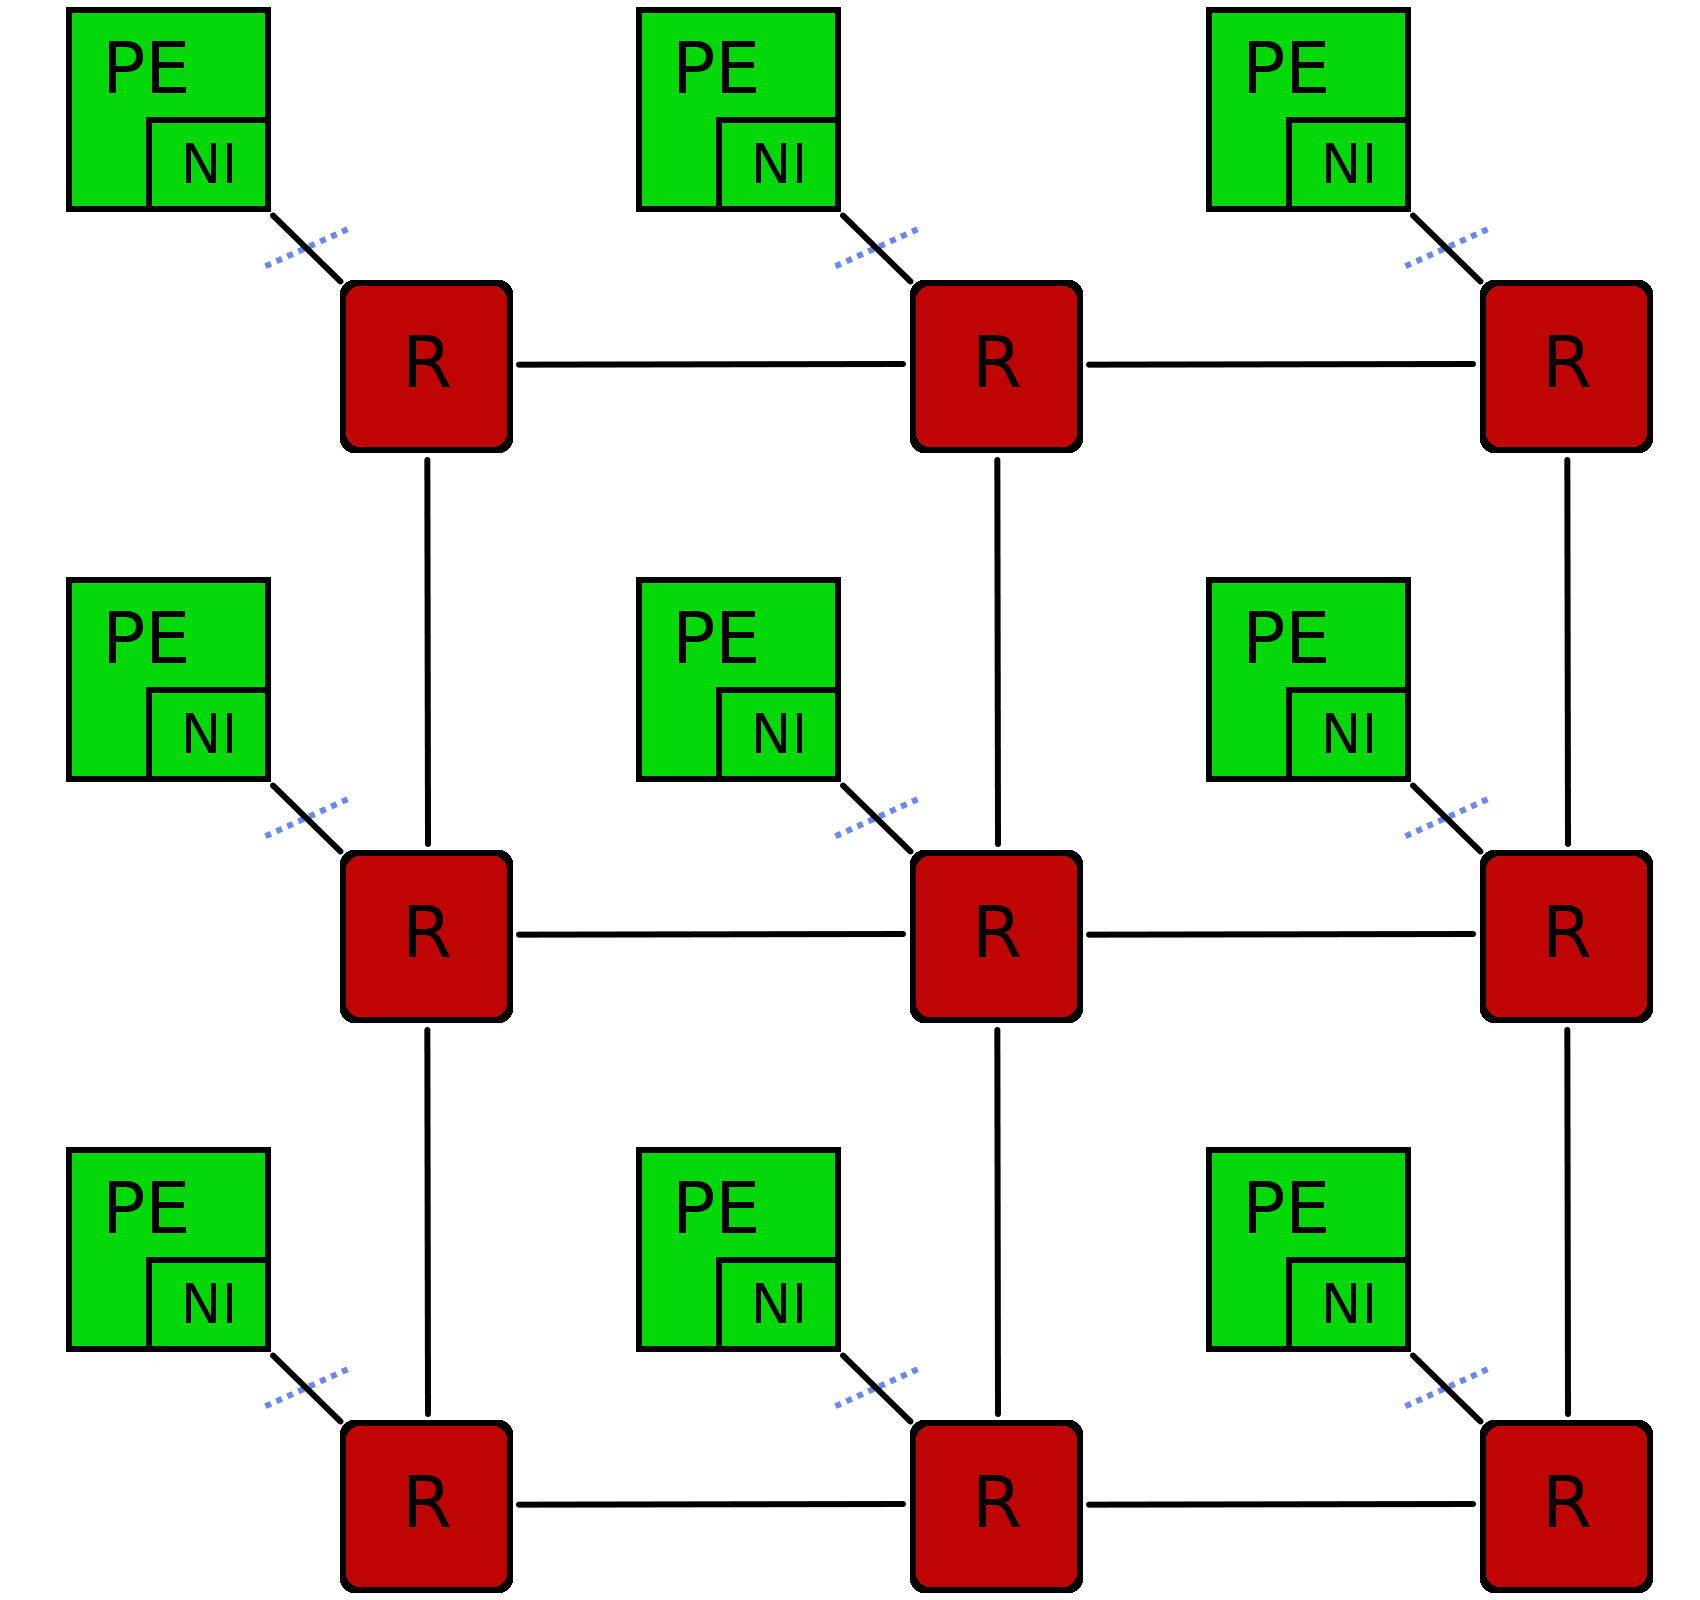
\includegraphics[width=0.5\textwidth]{noc-trust-boundaries}
    \caption[Trust boundaries in a NoC]{Visualization of the trusted and untrusted hardware components in a NoC. The processing elements and network
    interfaces, which are assumed to be trusted, are marked green. The network itself, which is comprised of the routers and their interconnections,
    is not trustworthy and thus marked red. The dotted lines at the local connections mark the trust boundaries.}
    \label{fig:noctrustboundaries}
\end{figure}

\section{Encryption And Authentication}\label{sec:encandauth}
The intent of integrating encryption and authentication is to provide confidentiality and integrity to messages passing through a \gls{noc}. To
implement this, a novel network interface design is proposed. Since all flits that enter the network must traverse one of the network interfaces,
they were chosen to host the cryptographic protection measures. In the proposed design, they encrypt all outgoing flits, which can only be decrypted by the
receiver. In addition, a \gls{mac} is computed that is sent together with the encrypted data. On the receiver side, the flits are decrypted and the
\gls{mac} is verified. This scheme is illustrated in Figure \vref{fig:nocflitencauth} and further explained in Section \ref{subsec:crypto}.

\begin{figure}
    \centering
    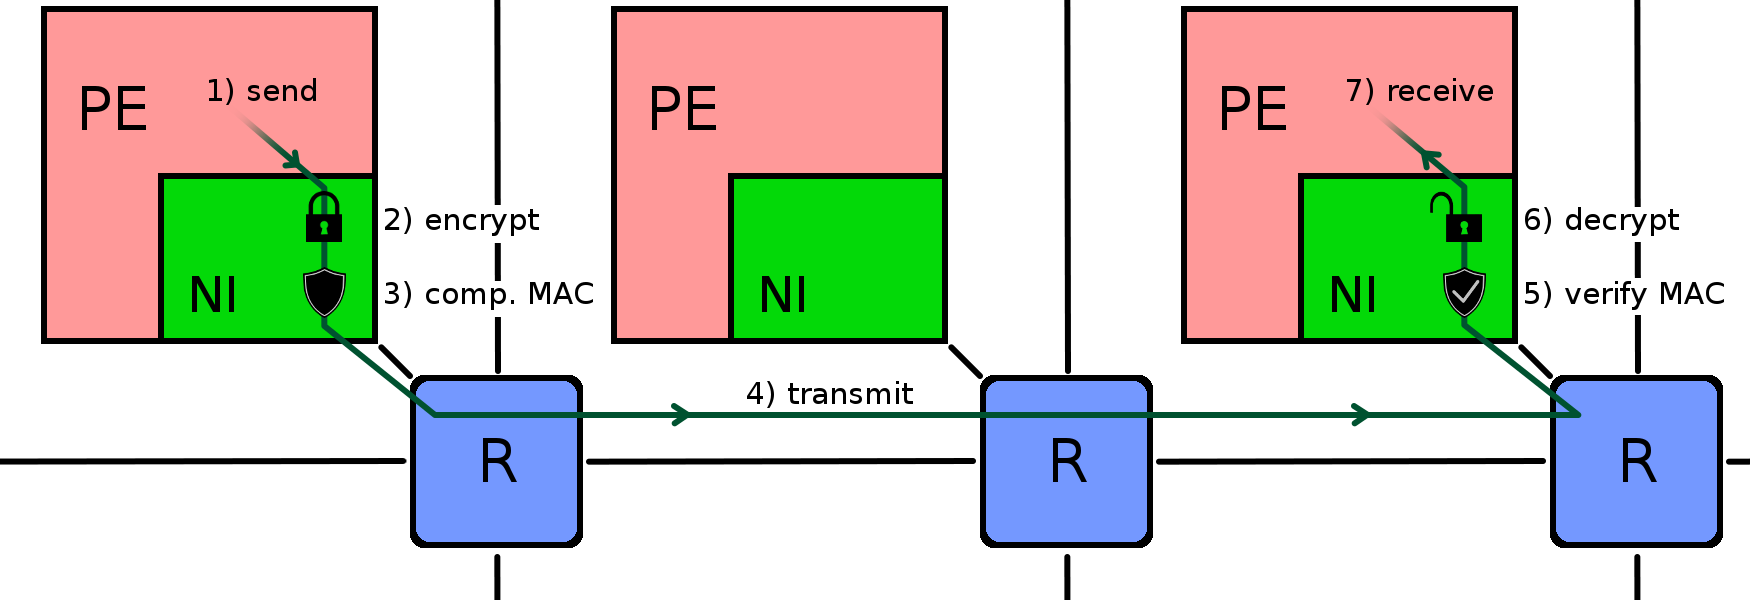
\includegraphics[width=0.9\textwidth]{noc-message-enc-auth}
    \caption[Flit in a NoC with encryption and authentication]{Example of a flit being transmitted through a NoC. After a processing element sends a flit (1),
    encryption is applied (2) and a MAC is computed (3) in the sender's network interface. The encrypted flit and the MAC are then routed to the
    destination (4). There, the receiver's network interface verifies the MAC (5) and decrypts the flit (6). Finally, the flit is passed to the
    receiving processing element (7). This scheme corresponds to the uncoded individual authentication protocol variant (see Section
    \ref{subsec:indauth} for details).}
    \label{fig:nocflitencauth}
\end{figure}

The constraints imposed by the \gls{noc} environment (cf. Section \ref{sec:networkonchipfun}) make the implementation of security measures a
challenging task. To meet them, only symmetric ciphers were investigated, as asymmetric ones imply high computational efforts
\cite[3]{moriam18activeattackers}. Furthermore, for authentication, they produce signatures that are \enquote{too long to be included in a flit}
\cite[3]{moriam18activeattackers}. In contrast, symmetric ciphers operate faster and allow for more compact implementations. Instead of
signatures, they employ \glspl{mac} that are short enough to fit into a single flit. However, the usage of symmetric ciphers implies that each pair of
sender and receiver needs to possess two shared secret keys (one for encryption and one for authentication). To obtain or renegotiate
such keys in a secure manner, a key exchange algorithm is required\footnote{One way to realize a secure key exchange in the context of \glspl{noc} is
the utilization of central key-keeper cores \cite{gebotys03securityframework} (see also Section \ref{subsec:securityzones}). Another option is
physical layer key generation, as suggested in the \gls{haec} presentation paper \cite[4]{matthiesen17haec}.}. As this exceeds the scope of this
thesis, each pair of sender and receiver is assumed to have access to the necessary keys.

\section{Network Coding}\label{sec:networkcodingover}
A promising approach to improve the performance of \glspl{noc} is network coding. \citeauthor{moriam15manycorenc} have shown that it is particularly
effective in error-prone networks, decreasing latencies by up to 95\% \cite[7]{moriam15manycorenc}. In the context of this thesis, \glspl{noc} are assumed
to be unreliable: compromised routers may deliberately inject faults or drop flits. Hence, this approach is taken up here to improve the network
performance.

While network coding provides robustness against sporadic flit loss, it does not offer any guarantees on the integrity of flits. Thus, modifications
during the transmission of the coded data are not detected directly, potentially leading to faulty decodings. This deficit is remedied by the cryptographic
layer described above. To evaluate the consequences of the integration of network coding, uncoded versions of the protocol were implemented and
examined as well (see Section \ref{sec:protocolvariants}).

\section{Multipath Routing}
The exploration of different routing strategies is a central aspect of this thesis. Both static and dynamic strategies were
examined and evaluated. With a static strategy, there is a predetermined, time-invariant path that a flit will take to reach a certain destination
from a particular sender. In contrast, dynamic strategies implement random factors that influence the routing decisions for each
transmission. Thus, even for the same pair of sender and receiver, different flits may take different paths through the network. The emphasis of this
thesis lies on dynamic strategies in order to capture the envisioned benefits of multipath routing.

As a deterministic strategy, \textit{dimension order routing (\gls{dor})} is used. On the dynamic side, \textit{dynamic minimal (\gls{dm})},
\textit{randomized oblivious multi-phase minimal (\gls{romm})}, and \textit{randomized adaptive multi-phase minimal (\gls{ramm})} routing are
explored. The properties and details of these strategies are presented in depth in Section \ref{subsec:routingstrategies}.

\section{Reliability}\label{sec:reliability}
In case the proposed techniques fail to achieve flawless transmission of a flit, it is crucial to provide a method for requesting
its retransmission. This occurs when the integrity check via \gls{mac} verification fails, indicating a modification in one or more of the
associated flits. Furthermore, when not enough flits arrive at the destination in time to perform the verifications in the first place, it is
necessary to request the retransmission of the missing ones. With network coding, at least partially intact transmissions are required, while an
uncoded scheme necessitates every flit to arrive unblemished.

The functionality for retransmissions is integrated into the protocol by means of \glspl{arq}. If one or more of the aforementioned events occur, the affected
receiver will issue an \gls{arq} back to the sender, who will then resend the flits in question.

To render retransmissions possible, a copy of each flit that is sent through the network is kept by the sender in order to answer a potential
\gls{arq} arriving later on. This is facilitated by a retransmission buffer that is included in every network interface. Each flit that is sent to the
network (except for the \glspl{arq} themselves) must pass through this buffer, where a copy of it is stored. When an \gls{arq} arrives from another
node, the requested flits are retrieved from the buffer and resent. As the retransmission buffer can only hold a finite number of flits, old ones are
replaced in a \gls{fifo} manner once maximum size is reached.

\section{Protocol Variants}\label{sec:protocolvariants}
To unearth and analyze the most efficient way of applying the ideas outlined above, different variants of the protocol were implemented. They differ
in the way the authentication \glspl{mac} are included in the flit transmissions. Furthermore, network coded and uncoded versions are compared to
examine the effects of network coding in combination with the cryptographic procedures. The emphasis of this thesis, however, is put on the network
coded forms.

The examined variants are \textit{individual authentication}, \textit{interwoven authentication}, and \textit{full-generation authentication}. For the
first two, both uncoded and network coded variants are implemented. For the latter, only a network coded version is feasible as the authentication
scheme relies on the existance of generations. A comprehensive description of all variants is given in Section \ref{sec:theprotocol}.

\section{Analysis And Evaluation}
All of the aforementioned protocol variants were implemented to empirically determine their quality and suitability for the task at hand. Many
experiments were conducted through software simulation of an \gls{mpsoc} with a \gls{noc} using varying parameters, component layouts, and design
decisions.

The experiments were performed with a simulator specifically crafted for this thesis. Based on the free and open source framework \textit{\omnet{}}
\cite{omnet}, it allows for cycle-accurate simulations with fully customizable statistics recording. Furthermore, its modular design allows for
quickly swapping and reordering the internal components of the network interfaces, which is a great asset for testing the different protocol variants.
The details of the implementation are described in Chapter \ref{ch:implementation}.

The workflow of the evaluation was as follows: at first, the hyperparameters\footnote{The term \textit{hyperparameters} refers to those parameters
whose value is determined through a number of preliminary experiments and remains static for the main experiments.} were
calculated which include, e.g., the number of required parallel crypto modules\footnote{The term \textit{crypto modules} is
used to refer to both encryption and authentication modules.} per network interface and the \gls{arq} timeouts. Afterwards, the remaining parameters are
varied to find the optimal configuration for each protocol variant. Finally, the most promising of these variants is identified. The full evaluation
process is elaborated in Chapter \ref{ch:evaluation}.


    \chapter{Communication Protocol}\label{ch:protocol}
    To accomplish the goals 

This chapter will illuminate the details of how encryption, authentication, network coding, and ARQ management are implemented in the network
interfaces.

Recall that the architecture of a \gls{noc} consists of a router grid with each node connected to a local processing element through a network
interface (cf. Figure \vref{fig:nocexample}). The 

There are different variants of the protocol, which are explained in detail in Section (insert vref here). While the emphasis lies on network coded
variants, uncoded versions have also been implemented for comparison purposes. However, not all methods have a corresponding uncoded variant.
% TODO: this goes to the overview chapter

Over the course of this chapter, the design of the communication protocol in all variants will be thorougly explained. To begin, fundamental
assumptions about the environment and basic building blocks of the protocol are presented. Since the protocol variants share many elements and differ
mostly in the authentication scheme, the simplest one (uncoded individual authentication) is used to give a step-by-step explanation of the full
protocol. Following this, the other variants are described by drawing upon the differences to uncoded individual authentication.

\section{Design Considerations}
\subsection{Flit Structure}
% Figure of the flit (bar) with header fields (for coded+uncoded)
% Explain purpose of header fields

\subsection{ARQ Structure}

\subsection{Network Coding}\label{sec:designnc}
The coding scheme used in this work slightly differs from the one described above. First, it is applied to unicast transmissions, while traditional
network coding focuses on multicast scenarios \cites{ahlswede00networkflow}{li03linearnc}. Second, only the sender nodes will compute combinations of
different flits, while intermediate nodes merely forward them. The rationale behind this are the tight performance requirements of \glspl{noc}. If
each network node waited for enough flits to perform local encoding before forwarding, routing latencies would increase. Furthermore, the
implementation of local encoding implies additional logic in each router, making their design more complex and entailing a higher chip area
requirement. However, this directly contradicts the \gls{noc} design goals laid out in Section \ref{sec:networkonchipfun} and is thus not considered.
% Only the sender codes
% TODO: mention PNC paper, that we use RLNC, but only senders encode and create generations ("only intra-session network coding")
% TODO: a bit of math and formulas on how NC is done (inspired by previous TUD papers)
% 2 sub-variants: G2C3, G2C4
% Why G2C3 and G2C4? → refer to previous TUD papers

\section{The Protocol}\label{sec:theprotocol}
As mentioned in Section \ref{sec:protocolvariants}, three different communication schemes were envisioned, with the first two subdivided into uncoded
and network coded versions. The remainder of this section provides a comprehensive specification of all variants.

\subsection{Individual Authentication}
\begin{figure}
    \centering
    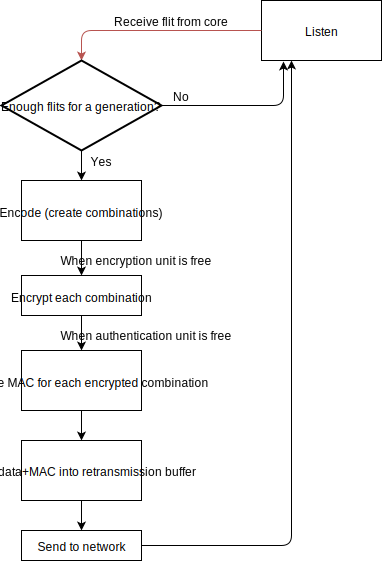
\includegraphics[width=\textwidth]{protocol-flowchart-nc-1}
    \caption[Protocol flow: method 1 coded]{Protocol flow: method 1 coded}
    \label{fig:protchartnc1}
\end{figure}
% uncoded (full explanation), network coded

\subsection{Interwoven Authentication}

\subsection{Full-Generation Authentication}

\section{Routing Strategies}
Mention the perceived/envisioned advantages of adaptive routing (different paths for each flit within the same sender-receiver pair → thanks
to NC enough flits will arrive hopefully even if one path contains a corrupted router).

\subsection{Deterministic XY}
The term \enquote{XY routing} stems directly from the behavior of the routers: flits are only routed along the X axis until they arrive in the column
that the receiver lies in, at which they are routed along the Y axis until reaching the receiver node.
% TODO: figure with a 2D mesh, X and Y arrows on the sides, example path marked for a transmission
\subsection{Dynamic Smart Random}
\subsection{Randomized Oblivious Multi-phase Minimal}
% Both with XY phases and DSR phases
This strategy essentially splits the routing problem into two phases: find a path from sender to proxy node and from proxy to receiver. For each
phase, one of the aforementioned strategies can be applied as is.

\begin{itemize}
    \item Routing Strategies
        \begin{itemize}
            \item Mention routing is general, we are special case of 2D mesh with uniform edge weights → much simpler than arbitrary networks
            \item XY/YX
                \begin{itemize}
                    \item Deterministic path
                    \item Attacker controlling a single router can reliably disrupt communication between certain nodes
                    \item does not distribute flits of a generation across different paths
                \end{itemize}
            \item XY/YX + Valiant
                \begin{itemize}
                    \item Deterministic path only if fixed valiant
                \end{itemize}
            \item Random XorY
            \item Random XorY + Valiant
            \item When writing about this: MANHATTAN DISTANCE (same for XY, YX, random XY, ROMM)
            \item Terminology:
                \begin{itemize}
                    \item Static=deterministic vs. dynamic (one fixed source-destination route or not)
                    \item Oblivious vs. adaptive (take into account network state or not)
                    \item Source routing: source decides a path, this is inserted into flit as metadata
                    \item ROMM is oblivious, use own term RAMM (randomized adaptive multi-phase minimal) for other variant
                    \item ROMM: oblivious, dynamic
                    \item DOR (dimension order routing): oblivious, deterministic
                \end{itemize}
        \end{itemize}
\end{itemize}

\iffalse
\section{Notes}
\begin{itemize}
    \item Encryption/authentication ordering
        \begin{itemize}
            \item Encrypt-then-MAC: best practice. Sequential encrypt/authenticate on sender side, but parallel decrypt/verify
                on receiver side. Advantage: MAC can be computed on receiver side immediately when ciphertext arrives, even when
                MAC flit has not arrived yet (if ARQ is necessary, it can be issued right away)
            \item MAC-then-encrypt: bad. Sequential authenticate/encrypt on sender side and sequential decrypt/verify on receiver
                side.
            \item Encrypt-and-MAC: okay. Parallel encrypt/authenticate on sender side, but sequential decrypt/verify on receiver
                side (overall same latency as Encrypt-then-MAC, but without advantage of fast ARQs)
        \end{itemize}
    \item Uncoded transmission
        \begin{itemize}
            \item no network coding
            \item 2 methods: 1 data flit + 1 MAC flit OR 2 data/MAC split flits
        \end{itemize}
    \item Flit structure
        \begin{itemize}
            \item burst bit, source/target address, mode, address, GID/FID, GEV, payload
            \item mode: define if data/mac/split/arq
        \end{itemize}
    \item Network coded transmission
        \begin{itemize}
            \item Number of flits: G2C3 or G2C4
            \item 3 methods: 1 data flit + 1 MAC flit OR 1 MAC flit per generation OR 2 data/MAC split flits
            \item mention that coded clits are slightly larger due to GEV being embedded → requires wider lanes
        \end{itemize}
    \item ARQs
        \begin{itemize}
            \item Limited number of ARQs per transmission unit (UC: data/MAC pair or split pair, NC: generation)
            \item Timeout of x (e.g. 8) cycles until first ARQ is sent
            \item If limit >1: start larger timeout (→ round-trip of ARQ)
            \item Many different cases, insert some flow diagrams here
            \item The higher the ARQ timeout/limit, the less likely the flit is still in retransmission buffer
            \item → ARQ timeout/limit and retransmission buffer size have to correlate
            \item In the case that we only have 1 ARQ left that we are allowed to send: Wait for any ongoing MAC verifications
                so in case they fail, the flits can be included in the ARQ
        \end{itemize}
\end{itemize}
\fi


    \chapter{Implementation}\label{ch:implementation}
    Following the design phase, it is crucial to test the protocol in a practical environment in order to verify that it works as intended. Furthermore,
extensive performance evaluations need to be conducted to assure the viability of the devised techniques. Both of these tasks are achieved through
software simulation. For this purpose, a dedicated, cycle-accurate simulator was developed that supports the designed protocol with all the
features described in Chapter \ref{ch:protocol}. A small portion of the codebase was already implemented before this thesis at the TU Dresden
Chair of Privacy and Data Security. However, most of it was refactored and the vast majority of the source code was written from scratch.

The simulator is implemented in C++ and based on the \textit{\omnet{}} discrete event simulation framework \cite{omnet}. \omnet{} provides a general-purpose
network simulation architecture and promotes a modular design. In general, it allows the programmer to define the components of the network via a
special scripting language called \textit{Network Description (NED)}. With NED files, the network's modules are specified as they appear from the
outside, by means of parameters,
gates, and connections. Furthermore, a module is allowed to have any number of submodules, facilitating a hierarchical structure. A C++
class is assigned to each module that defines its internal behavior based on the given parameters. The gates define the communication interfaces of the
module through which it sends and receives messages. The connections link the gates of different modules (or submodules) together and thus define the
message flows and the network's topology.

The simulator makes extensive use of the hierarchical and modular approach of \omnet{}. The processing elements, network interfaces, and routers are
defined as modules and instanced as many times as required, depending on the \gls{noc} dimensions. They are interconnected through their gates and
arranged in a way mirroring the structure of the \gls{noc}. To create a simulation as realistic as possible, they are made up of a number of
submodules, such as queues, buffers, and crypto modules, resembling the actual hardware layout.

\omnet{} allows the user to freely implement detailed statistics to be recorded during simulations. They provide the foundation for the evaluation
in Chapter \ref{ch:evaluation}. Data sets are obtained by running numerous simulations with varying configurations.

In Section \ref{sec:generalass}, fundamental assumptions about the simulation environment are presented. Subsequently, Section
\ref{sec:componentstructure} elaborates on the hierarchical structure of the components and their layout. Finally, an overview of the internal delays
and latencies that the various submodules entail is given in Section \ref{sec:internaldelays}.

\section{General Assumptions}\label{sec:generalass}
\subsection{Globally Synchronous Architecture}
In Section \ref{sec:networkonchipfun}, it was mentioned that \glspl{noc} lend themselves well to the implementation of the \gls{gals} design paradigm.
For the simulation, it was not considered for three reasons. First, its usage requires the existance of multiple clock domains: each core runs with the
frequency best suited for itself and is not synchronized with other cores in the network (\enquote{globally asynchronous}). This, however, is very
cumbersome to implement correctly. Second, since the cores themselves each operate under a single clock (\enquote{locally synchronous}), \gls{gals} would
only affect the transmissions from one router to another. Third, the cores are assumed to be identical and hence run with the same frequency anyway.
On these grounds, a globally synchronous architecture with a single clock driving all components is used in the simulator.

\subsection{Clock Frequency}\label{subsec:clockfrequency}
The \gls{noc}'s global clock runs at a frequency of 500 MHz as this is a common speed in \gls{noc}-related research
\cites{frey15stateobfuscation}{frey17hardenednoc}{haas18sdrmpsoc}. Unfortunately, the PRINCE cipher that is employed for all cryptographic operations
is unable to run at
such a high frequency. However, in Section \ref{subsubsec:prince} it was shown that the algorithm runs flawlessly at frequencies of up to 250 MHz.
Thus, the crypto modules operate at half the frequency of the \gls{noc}, with every two cycles of the global clock corresponding to one
cycle for the crypto modules. Hence, the processing of a single block with PRINCE is assumed to take two clock cycles in the simulator.

It was mentioned above that the integration of multiple clock domains is intricate. However, when they are not independent and the global clock's
frequency is evenly divisible by the target frequency, as is the case for the crypto modules, this becomes significantly easier. Here, a new clock
is derived from the global clock that simply omits every other tick.

\subsection{Single Cycle Routing}\label{subsec:singlecyclerouting}
The number of cycles required for routing\footnote{Routing refers to the whole process from receiving a flit on an input port to forwarding it on the
appropriate output port, including route calculation, switch allocation, and switch traversal \cite[see][2]{routinglectureutah}. These computations
are performed by every intermediate node along a flit's path.} is a key factor to the
overall performance of the \gls{noc}. While four cycle \cite[e.g.][]{routinglectureutah} and two cycle routing \cite[e.g.][]{lu11nocrouter} are
popular approaches, architectures requiring only a single cycle have also proven to be both feasible and practical
\cites{hayenga09scarab}{ved17routeonfly}.

As achieving low latencies is of utmost importance for this thesis, single cycle routing is implemented in the simulator. Such an approach is easily
able to operate at the required frequency of 500 MHz \cite[7]{hayenga09scarab}. Furthermore, high routing speeds imply less required buffers
\cite[1]{ved17routeonfly}, reducing the occupied chip area of the routers. Although completely bufferless architectures are possible
\cite{hayenga09scarab}, the implemented scheme grants each router one input buffer per port (i.e., five buffers per router) in order to prevent
flits from being discarded if they cannot be forwarded immediately. Their sizes are one of the hyperparameters of the simulator and are determined in
Section \ref{subsec:portqueuesizes}. Output buffers are not used in the routers.

In order for the complexity of the simulator to stay within manageable bounds, the internal structure of the routers is kept simple. For instance, no
virtual channels\footnote{When the physical connections between routers are multiplexed onto multiple virtual ones with separate input
buffers, this is referred to as virtual channels.} are used for the input buffers mentioned above. This, however, implies that a flit delayed by a
congestion of the targeted output
link also holds back all following flits in the buffer, even if they would be routed to a different link.

\subsection{Retransmission Buffer}
In Section \ref{subsec:arqretransmissions}, it was mentioned that \glspl{arq} are not authenticated. This implies that there is no method to ensure
the integrity of \glspl{arq}. However, the worst case scenario is that a modified \gls{arq} causes different flits to be retransmitted than the
intended ones, entailing unnecessary network load. To simplify this case, a modified \gls{arq} is ignored by the \gls{rtb}.

\section{Component Structure}\label{sec:componentstructure}
This section provides an in-depth view on the modular structure of the simulator. In a top-down approach, it begins with the outermost layer of the
hierarchy (i.e., the \gls{noc} itself) and then descends into the individual components. The figures used to support the textual explanations are
drawn directly from the graphical interface provided by \omnet{}.

\subsection{Complete Network}
The structure of the \gls{noc} in the simulator mirrors the 2D mesh topology of the network (cf. Figure \ref{fig:nocexample}). The only difference
here is that the network interfaces are not built as submodules of the processing elements, but as independent components interposed between the
processing elements and routers. Figure \vref{fig:omnetnoc} visualizes this approach.

\begin{figure}
    \centering
    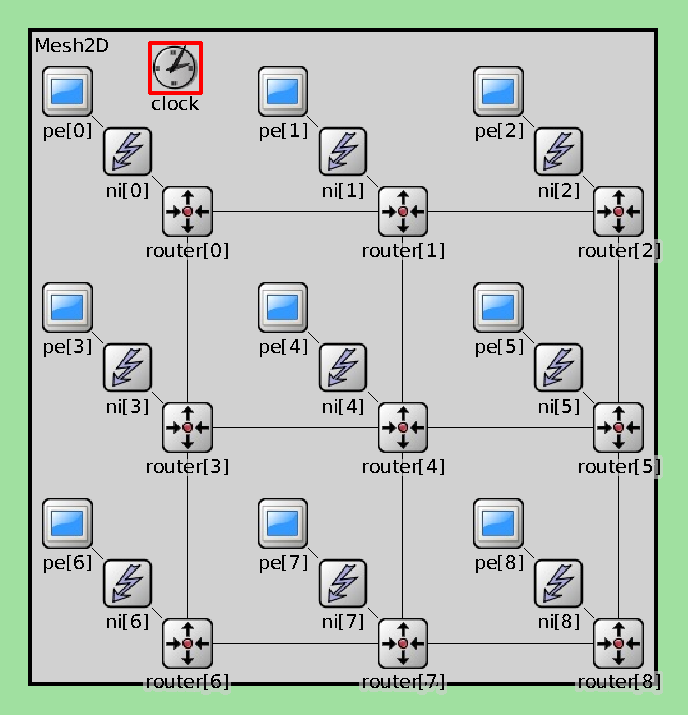
\includegraphics[width=0.5\textwidth]{omnet-noc}
    \caption[Simulator view of the NoC]{The \gls{noc} as it appears in \omnet{}. For clarity reasons, it was truncated to a 3x3 mesh. Each processing
    element, network interface, and router are assigned an index for simulation purposes. The network interfaces were not integrated into the
    processing elements to allow for better visualizations of the traffic flow.}
    \label{fig:omnetnoc}
\end{figure}

In addition to these familiar components, the global clock is also implemented as its own module. As a part of the simulation, it drives all other
modules and their submodules through signals. Any module may attach itself to this clock by registering as a receiver for the appropriate signal.

\subsection{Processing Element}
The processing element is a very plain component from the perspective of the simulator. It contains nothing more than a traffic generator and a flit
consumer with an input queue. Figure \vref{fig:omnetpe} depicts its appearance in \omnet{}.

\begin{figure}
    \centering
    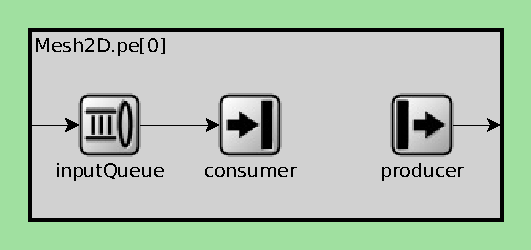
\includegraphics[width=0.5\textwidth]{omnet-pe}
    \caption[Simulator view of the processing element]{An instance of a processing element module of \omnet{}. A traffic generator (producer) randomly
    creates flits and sends them to the connected network interface. Flits arriving from the network interface are accepted by a pseudo-buffer
    (inputQueue) that subsequently passes them to the consumer.}
    \label{fig:omnetpe}
\end{figure}

The traffic generator randomly produces flits and sends them to the network interface\footnote{This traffic generation scheme was adopted from
\citeauthor{moriam18activeattackers} \cite{moriam18activeattackers}.}. On each clock tick, one flit is created with a configurable
\textit{generation probability}. The destination is chosen at random from the set of network nodes (excluding the own node) with a uniform
distribution. The produced flits are always data flits (not \glspl{mac} or \glspl{arq}) without any meaningful information contained in their
payloads\footnote{For the simulation, only the transmission parameters are of interest, not the actual data being transferred.}. Furthermore, the
generator may be configured to always produce a pair of two flits: in the event of a flit creation as described above, another flit will always be
produced on the next clock tick with the same destination. The purpose of this generation pattern is to allow for a fair comparison of uncoded and
network coded protocol variants. A detailed explanation is given in Section \ref{sec:environmenteval}.

The flit consumer simply accepts any flits arriving from the local network interface and records these events with \omnet{}'s statistics system. Since
the flits are of no further use after this, they are subsequently destroyed. An input buffer is located in front of the consumer to ensure both
synchronization with the global clock and that the travel time from network interface to processing element is precisely one cycle.

\subsection{Network Interface}
The network interface is the most complex part of the simulator. Implementing all the logic required by the protocol, it contains several crypto
modules, network coding components, the retransmission buffer as well as the verification and \gls{arq} infrastructure. The layout of these components
slightly differs for each variant. However, all variants resemble the structure of their corresponding flowchart in Section \ref{sec:theprotocol}, so
explaining the network interface by means of one variant is deemed sufficient. For this purpose, the network coded interwoven authentication version
is described below. Figure \vref{fig:omnetni} shows the internal structure as rendered by \omnet{}'s graphical interface.

\begin{figure}
    \centering
    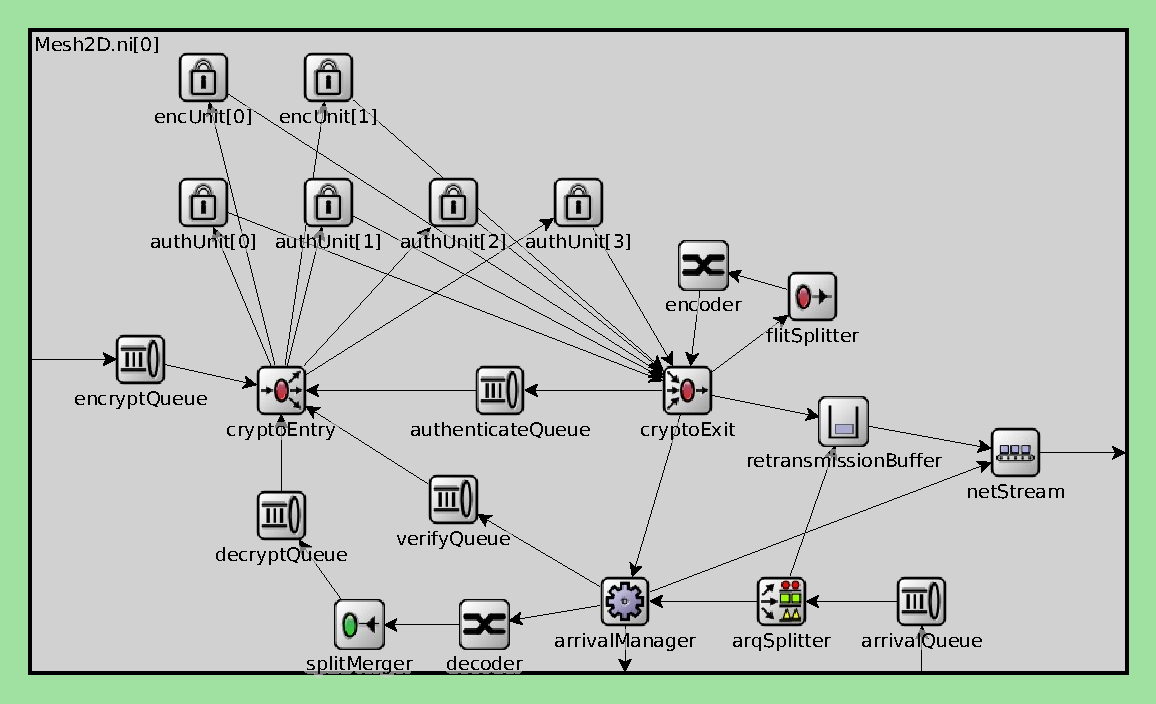
\includegraphics[width=0.85\textwidth]{omnet-ni}
    \caption[Simulator view of the network interface]{An instance of a network interface for network coded interwoven authentication as rendered by
    \omnet{}. Flits from the processing element arrive on the left side and subsequently traverse a pipeline of encryption, encoding, and
    authentication modules. The flits from the router enter the interface on the bottom right. After \glspl{arq} are filtered out, the remaining flits
    are subjected to decoding, decryption, and verification procedures before being forwarded to the processing element.}
    \label{fig:omnetni}
\end{figure}

The network interface was modeled as accurately as possible to facilitate detailed statistics about the flit flow inside them. This allows for the
evaluation of internal delays that are caused, for instance, by departing and arriving flits competing over the available crypto modules, or a
retransmission competing with a new flit over the link to the router. Thus, the implementation of the network interfaces consists of a number of
different submodules, and flits take rather intricate paths through them. In the following sections, the progression of an exemplary transmission unit
both for departing (\gls{pe} $\rightarrow$ router) and arriving (router $\rightarrow$ \gls{pe}) flits is given.

\subsubsection{Path Of Departing Flits}
Flits entering the network interface from the processing element are first placed into a queue (\textit{encryptQueue} module on the left side of
Figure \ref{fig:omnetni}). As the name suggests, they wait here for an encryption module to become available. Once this is the case, the front
flit is fetched from the queue and redirected to the appropriate encryption module.

The network interface's crypto modules are managed by an auxiliary module (named \textit{cryptoEntry} in Figure \ref{fig:omnetni}). It keeps track of
the availability status of both the encryption and the authentication modules and handles the distribution of flits among them. There are multiple
queues connected to it; the aforementioned \textit{encryptQueue} and three others whose role will be explained below. It should be noted that only one
flit can be fetched from each queue per clock cycle. In the current path of the exemplary flit, \textit{cryptoEntry} will fetch it from
\textit{encryptQueue} once one of the encryption modules (named \textit{encUnit} suffixed with an index in Figure \ref{fig:omnetni}) becomes
available.

Once the encryption module has finished its task, the flit arrives at another auxiliary module where the paths from all crypto modules converge.
Aptly named \textit{cryptoExit} in Figure \ref{fig:omnetni}, incoming flits are redirected depending on their arrival gate. For the current case, the
encrypted flit is sent to the \textit{flitSplitter}.

With the interwoven authentication protocol variant, the next step is to create a new flit that half the payload is moved to. Afterwards, these two
flits are encoded as a generation by the \textit{encoder}. The resulting three or four flits are subsequently sent back to the \textit{cryptoExit}
auxiliary module which merely forwards them to the \textit{authenticateQueue}\footnote{The flits could also bypass the \textit{cryptoExit} and head
straight for the \textit{authenticateQueue}, but this would have been more tedious to implement. The forwarding by \textit{cryptoExit} imposes no
temporal overhead.}. As the computation of a combination takes one clock cycle, the encoder
consequently sends out precisely one combination per cycle.

Now, each combination needs to be authenticated. The \textit{authenticateQueue} is one of the four queues connected to the \textit{cryptoEntry}. In
the same manner as for the encryption process, \textit{cryptoEntry} fetches the front flit from the \textit{authenticateQueue} once one of the
authentication modules (referred to as \textit{authUnit} suffixed with an index in Figure \ref{fig:omnetni}) is available and forwards it
appropriately.

When the authentication process is complete, the flits once again arrive at the \textit{cryptoExit}. This time, however, they are forwarded to the
\textit{retransmissionBuffer}. Here, each one is copied as specified in the protocol before being sent to the network. The \textit{netStream} is
another auxiliary module that merely serializes departing flits, retransmissions, and issued \glspl{arq} in case they arrive here at the same clock
cycle. This is necessary since multiple flits cannot occupy the link to the router at the same time.

\subsubsection{Path Of Arriving Flits}
When a flit arrives from the network, it is first placed into a queue (named \textit{arrivalQueue} and located at the bottom right of Figure
\ref{fig:omnetni}). However, flits are only kept here until the next clock tick. The purpose of this procedure is to ensure that the travel time from
the router was precisely one clock cycle.

The next station is the \textit{arqSplitter} supplementary module. Its only task is to check the incoming flit's mode field. In case of an
\gls{arq}, it is sent straight to the \textit{retransmissionBuffer} which subsequently performs the appropriate retransmissions. Otherwise, the flit
is forwarded to the \textit{arrivalManager}.

The \textit{arrivalManager} is the most complex submodule of the network interface. It buffers incoming flits, performs verifications through authcode
comparisons, and keeps track of the \gls{arq} timeouts for all the transmission units. For each arriving flit, two copies are made: one to compute an
authcode over and one for decoding and decryption.

While the original is stored for the upcoming verification process, the first copy is sent to the
\textit{verifyQueue}, which is connected to the \textit{cryptoEntry}. Identically to the departing flits waiting for authentication, the
\textit{cryptoEntry} fetches flits from the queue once an authentication module is available. However, in case there are flits in both the
\textit{authenticateQueue} and the \textit{verifyQueue}, the former always takes priority\footnote{The rationale for preferring departing flits is to
not disperse generations that will be sent to the network. If the flits are already spaced out when leaving the interface, the probability for causing
unnecessary \gls{arq} timeouts increases needlessly.}.

The second copy is forwarded to the decoder. It is buffered here until another flit from the
same transmission unit arrives. Both are subsequently decoded and merged back into a single flit, which is then sent to the \textit{decryptQueue}. As
the name suggests, the flit stands by until the \textit{cryptoEntry} has allocated an encryption module for it\footnote{As laid out in Section
\ref{subsubsec:prince}, the encryption modules are able to perform decryptions as well.}. Corresponding to the authentication process, departing flits
take priority over the encryption module access when both \textit{decryptQueue} and \textit{encryptQueue} are not empty. Both the decrypted flits and
computed authcodes are redirected back to the \textit{arrivalManager} by the \textit{cryptoExit}. Authcodes are compared with those contained in the
originally buffered flits; in case of their equality, the decrypted flit is sent directly to the processing element.

In case an \gls{arq} must be issued, either caused by non-equal authcodes or timeouts, the \textit{arrivalManager} generates and prepares an
\gls{arq} flit. From there, it is sent to the network via the \textit{netStream} auxiliary serialization module.

\subsection{Router}\label{subsec:routerimpl}
Like the processing elements, the routers' internal structure is straightforward. Presented in Figure \vref{fig:omnetrouter}, it consists of a switch
and five input buffers (one for the local network interface and four for the neighboring routers). These buffers are referred to as the \textit{local
queue} and the \textit{port queues}, respectively.

\begin{figure}
    \centering
    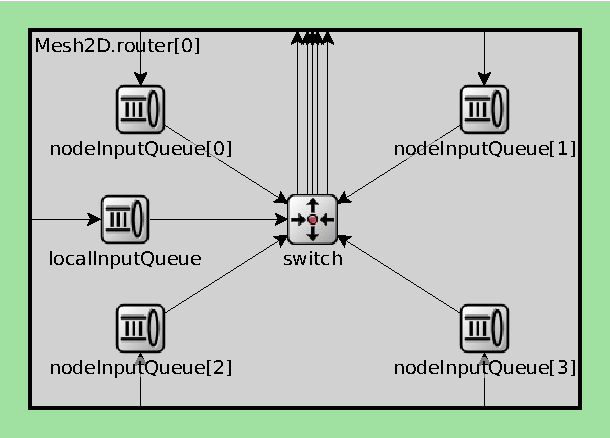
\includegraphics[width=0.55\textwidth]{omnet-router}
    \caption[Simulator view of the router]{An instance of a router as rendered by \omnet{}. The five input gates are connected to the switch via their
    input queues. The five respective output connections are not interposed by a buffer. In the renderings of \omnet{}, the spatial layout of the
    connections sometimes does not match their logical correlations, as is the case here with the output lines being drawn in parallel. However, there is
    in fact one output connection corresponding to each input gate.}
    \label{fig:omnetrouter}
\end{figure}

The routing logic is located within the switch submodule. On every clock tick, it checks the front flits in each queue and computes the most suitable
output ports for them. This computation (often referred to as \textit{route calculation}) depends on the flit's destination header and the implemented routing
strategy. If a calculated output port is unavailable due to the link being congested, the affected flits are delayed until the next clock tick.
Furthermore, in case multiple flits are to be routed through the same output port, one of them is randomly selected while the others are postponed.
Flits from different queues with differing output ports can be routed simultaneously.

Routers are able to inform neighboring ones of congestions of their input queues. Once a queue has reached a certain size, the router sends a congestion signal to the
neighbor connected to this queue\footnote{For instance, these notifications can be realized through dedicated signaling lines on the router
interconnections. This would increase the channel width from 141 to 142 wires and from 149 to 150 wires for uncoded and network coded protocols,
respectively (cf. Section \ref{subsec:flitstructure}).}, thereby instructing it to delay all flits that are supposed to be routed towards the
signaling router, if possible. Once the congestion has subsided, the affected neighbor is informed of this event through a similar signal and may
resume normal routing of flits in the affected direction.

\section{Internal Delays}\label{sec:internaldelays}
To elucidate the impact of each module on the overall processing latency, their delays are elaborated in this section.
Table \ref{tab:processinglatencies} presents the processing times for the submodules of the network interfaces, while Table
\vref{tab:transmissionlatencies} shows the transmission durations between the \gls{noc}'s components.

\begin{table}
    \centering
    \begin{tabulary}{\textwidth}{R|L}
        Procedure & Delay in cycles \\\hline
        Encryption/decryption & 2 \\
        Encoding (G2C3) & 3 (1 per combination) \\
        Encoding (G2C4) & 4 (1 per combination) \\
        Authentication (individual) & 6 \\
        Authentication (interwoven) & 5 \\
        Authentication (full gen.) & 10 \\
        Decoding & 2 (1 per flit) \\
        \gls{mac} comparison & 1 \\
        \gls{arq} composition & 1 \\
        Flit storage in \gls{rtb} & 1 \\
        \Gls{rtb} lookup & 1 (uncoded), 2 (network coded)
    \end{tabulary}
    \caption[Internal computation delay in the network interface]{Internal computation delays of various procedures within the network interfaces.}
    \label{tab:processinglatencies}
\end{table}

\begin{table}
    \centering
    \begin{tabulary}{\textwidth}{R|L}
        Transmission & Delay in cycles \\\hline
        PE $\Leftrightarrow$ NI & 1 \\
        NI $\Leftrightarrow$ Router & 1 \\
        Router $\Leftrightarrow$ Router & 1
    \end{tabulary}
    \caption[Transmission latencies for the NoC interconnections]{Transmission latencies of the \gls{noc} interconnections. The inter-router
    communication includes the route calculation and switching process in the originating router.}
    \label{tab:transmissionlatencies}
\end{table}

The delay for the encryption and decryption is precisely two clock cycles for all protocol variants as exactly one input block (the flit payload)
needs to be processed. For authentication, the number of input blocks (and consequently the delay) varies. With individual authentication, three
blocks are processed, corresponding to six clock cycles. Interwoven authentication only has two input blocks, but entails an additional cycle for the
authcode calculation. With full-generation authentication, the two input flits are divided into five blocks and thus require ten cycles of
processing.

The lookup procedure for the retransmission buffer works as follows: when an \gls{arq} arrives, the first action is to find the correct buffer
depending on the \gls{arq}'s source. As the location of each buffer is static, this does not require a dedicated clock cycle. Afterwards, the position
of the affected transmission unit inside the buffer needs to be identified by searching for the unit's ID, which takes one cycle. Finally, the
required flits are retrieved from the buffer using the modes specified in the \gls{arq}. Once the transmission unit's location is known, the position
of the individual flits is determined by fixed offsets from this location depending on the mode, which eliminates the need to search for each one.

Thus, for uncoded protocol variants, an \gls{rtb} lookup takes one clock cycle. However, if multiple flits need to be retransmitted, only one can be
sent out per cycle since the link to the router cannot be occupied by more than one flit at the same time.

In network coded environments, the mode header field does not suffice to uniquely identify a flit within a transmission unit; the \glspl{gev}
specified in the \gls{arq} need to be compared as well. Hence, a flit's position is determined by first finding the ID, then the affected \glspl{gev},
and finally the required modes for each \gls{gev}. This extended procedure adds one clock cycle to the lookup time for a total of two cycles.


    \chapter{Evaluation}\label{ch:evaluation}
    \section{Notation}
%Placeholder parameters
%Prot. variants abbreviations (IDA, IWA, FGA, UC) (G2C3 and G2C4 as before)
%Term "source flit"

\section{Environment}
% 50,000 cycles (why?)
% Warmup and cooldown times (both 500 cycles)
% Injection rate of 0.2 into the network
% TODO: Router queue sizes (no limit for local input queue to avoid flits being discarded for simulation purposes)
In the experiments, a base network injection rate of 0.2 is assumed. This is the same value that \citeauthor{moriam18activeattackers} have chosen
\cite[2]{moriam18activeattackers} in order for the results to be comparable with their analyses. The actual injection rate may be higher as the base rate does not include the
issuance of \glspl{arq} and the resulting retransmissions.
\begin{itemize}
    \item Injection rate
        \begin{itemize}
            \item Value if 0.2 is realistic
            \item Possibility to generate pairs for fair comparison of UC/NC
            \item Base network injection rate of 0.2 is used for all experiments. The source flit creation rate is adjusted accordingly for the
                protocol variants to ensure that they have the same injection rate.
        \end{itemize}
    \item Overhead von Verschlüsselung+Auth vs. nur Auth vs keins von beiden (sowohl Latenz als auch Chipfläche)
\end{itemize}

\begin{table}
    \centering
    \begin{tabulary}{\textwidth}{C|C}
        Parameter name & Value \\\hline
        \Gls{noc} dimensions & 8x8 \\
        Clock frequency & 500 MHz \\
        Network base injection rate & 0.2 \\
        Simulation runtime & \num{50000} cycles \\
    \end{tabulary}
    \caption[short]{long}
    \label{tab:fixedparams}
\end{table}

\begin{table}
    \centering
    \begin{tabulary}{\textwidth}{C|C|C}
        Parameter name & Value range & Placeholder \\\hline
        Network coding & $\{\mathit{UC}, \mathit{G2C3}, \mathit{G2C4}\}$ & \pNCMode{} \\
        No. of encryption modules & $\mathbb{N}^*$ & \pEncMods{} \\
        No. of authentication modules & $\mathbb{N}^*$ & \pAuthMods{} \\
        \Gls{arq} limit & $[1, 2]$ & \pARQLimit{} \\
        \Gls{arq} timeout & $\mathbb{N}^*$ cycles & \pARQTimeout{} \\
        Routing strategy & $\{\mathit{\gls{dor}}, \mathit{\gls{dm}}, \mathit{\gls{romm}}, \mathit{\gls{ramm}}\}$ & \pRStrat{} \\
    \end{tabulary}
    \caption[short]{long}
    \label{tab:inputparams}
\end{table}

\section{Attacker Model}
\begin{itemize}
    \item Focuses on malicious modifications rather than DoS attacks
    \item Assumption: compromised routers → rely on NIs for security
    \item No protection against bandwidth depletion, but this is not the goal here
    \item Variable number of compromised routers (e.g. 8 for an 8x8 grid)
    \item Compromised routers randomly drop or modify packets (no intelligent modifications/drops)
    \item Reasoning for having only some compromised routers (in regard to the 3rd party NoC problem → why would they not make all routers the same?)
        → HT implies more logic in routers → more area and draws more power → might attract attention if all routers have this and overall NoC
        parameters diverge considerably from the expectations
\end{itemize}

Compromised routers: 6, 8, 23, 36, 46, 52, 59, 61 (8 routers randomly selected from the set of nodes with uniform probability distribution)

\section{Determining The Hyperparameters}
\subsection{ARQ Timeouts}\label{subsec:arqtimeouts}
In Section \ref{subsec:arqretransmissions}, the concept of \glspl{arq} and timeouts was introduced: receivers issue \glspl{arq} when the temporal gap
between the arrival of flits belonging to the same transmission unit becomes too large, i.e. when a timeout occurs. Its value is determined through
experiments and measured in clock cycles.

\begin{figure}
    \centering
    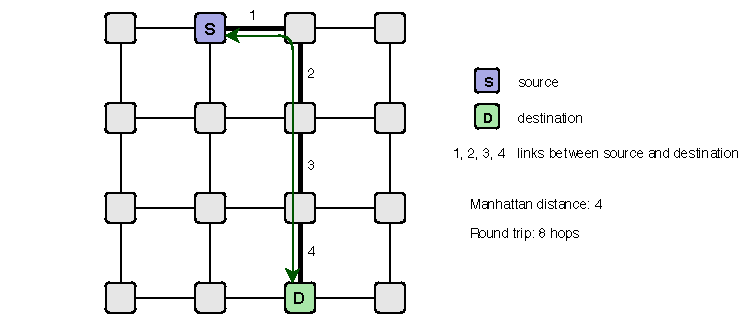
\includegraphics[width=0.9\textwidth]{arq-timeouts-calc}
    \caption[Example of ARQ timeout calculation]{Example for the calculation of \gls{arq} timeouts. With a Manhattan distance of 4 between source $S$ and
    destination $D$ and a given inter-arrival timeout $t_1$, the \gls{arq} timeout $t_2(S, D)$ is computed as $t_1 + 2 \cdot 4 = t_1 + 8$ cycles.}
    \label{fig:arqtimeoutscalc}
\end{figure}

In addition to the inter-arrival timeout, there is another, higher value that is used after an \gls{arq} was issued to await the answer, as explained
in Section \ref{subsec:arqretransmissions}. The \gls{arq} answer timeout depends on the inter-arrival timeout and the Manhattan distance between the
two affected communication partners. More precisely, if $t_1$ is the inter-arrival timeout, $t_2(S, D)$ is the \gls{arq} answer timeout for a
particular source $S$ and destination $D$, and $d$ is the Manhattan distance between the two nodes, then $t_2(S, D) = t_1 + 2 \cdot d$. Figure
\vref{fig:arqtimeoutscalc} illustrates this calculation.

Hence, only $t_1$ needs to be determined through experiments. Since this is the first parameter to be fixed, the other input values for the simulation
are estimated. The tests are independent of the protocol variant as the same injection rate is used for all of them. Table \vref{tab:setuparqtimeouts}
presents how the simulator is set up.

\begin{table}
    \centering
    \begin{tabulary}{\textwidth}{C|C|C|C|C|C|C|C|C}
        \pProtVar{} & \pNCMode{} & \pEncMods{} & \pAuthMods{} & \pARQLimit{} & \pARQTimeout{} & \pRStrat{} & \pNumAttackers{} & \pAttackProb{} \\\hline
        \gls{ida} & varying & 5 & 15 & 1 & varying & \gls{dor} & 0 & 0 \\
    \end{tabulary}
    \caption[Input parameters for ARQ timeouts experiment]{long}
    \label{tab:setuparqtimeouts}
\end{table}
% Why Ind. Auth.? Most flits per transmission unit (8 with G2C4)
% Why this number of enc./auth. units? Large number so there are definitely no internal congestions → area doesn't matter for this experiment
% Why ARQs per source flit and not per transmission unit? because size of trans. units varies considerably with prot. variant

To determine the timeout value, an uncompromised \gls{noc} (i.e., with zero malicious routers) is used. Ideally, no \glspl{arq} are issued in this
scenario. However, due to random deviations from the average flit injection rate, the network load varies over time and congestions in some routers
may occur. The resulting increased transmission delays may be high enough to trigger timeouts even when an \gls{arq} is not necessary. Sporadic
occurances of such cases cannot be ruled out, but should rarely happen. However, simply increasing the timeout until these cases vanish is undesirable
for two reasons. First, a high timeout directly corresponds to high latencies when flit losses necessitate \glspl{arq}. Second, the later an \gls{arq}
is issued, the larger the \gls{rtb} of the communication partner needs to be so that the flits in question are not already overwritten when the
\gls{arq} arrives. The goal of this experiment is to find a reasonable middle ground: the smallest timeout that does not entail a significant number of
unnecessary \glspl{arq} will be used for the subsequent evaluations.

\begin{figure}
    \centering
    % GNUPLOT: LaTeX picture with Postscript
\begingroup
\newcommand{\ft}[0]{\footnotesize}
  \makeatletter
  \providecommand\color[2][]{%
    \GenericError{(gnuplot) \space\space\space\@spaces}{%
      Package color not loaded in conjunction with
      terminal option `colourtext'%
    }{See the gnuplot documentation for explanation.%
    }{Either use 'blacktext' in gnuplot or load the package
      color.sty in LaTeX.}%
    \renewcommand\color[2][]{}%
  }%
  \providecommand\includegraphics[2][]{%
    \GenericError{(gnuplot) \space\space\space\@spaces}{%
      Package graphicx or graphics not loaded%
    }{See the gnuplot documentation for explanation.%
    }{The gnuplot epslatex terminal needs graphicx.sty or graphics.sty.}%
    \renewcommand\includegraphics[2][]{}%
  }%
  \providecommand\rotatebox[2]{#2}%
  \@ifundefined{ifGPcolor}{%
    \newif\ifGPcolor
    \GPcolortrue
  }{}%
  \@ifundefined{ifGPblacktext}{%
    \newif\ifGPblacktext
    \GPblacktextfalse
  }{}%
  % define a \g@addto@macro without @ in the name:
  \let\gplgaddtomacro\g@addto@macro
  % define empty templates for all commands taking text:
  \gdef\gplbacktext{}%
  \gdef\gplfronttext{}%
  \makeatother
  \ifGPblacktext
    % no textcolor at all
    \def\colorrgb#1{}%
    \def\colorgray#1{}%
  \else
    % gray or color?
    \ifGPcolor
      \def\colorrgb#1{\color[rgb]{#1}}%
      \def\colorgray#1{\color[gray]{#1}}%
      \expandafter\def\csname LTw\endcsname{\color{white}}%
      \expandafter\def\csname LTb\endcsname{\color{black}}%
      \expandafter\def\csname LTa\endcsname{\color{black}}%
      \expandafter\def\csname LT0\endcsname{\color[rgb]{1,0,0}}%
      \expandafter\def\csname LT1\endcsname{\color[rgb]{0,1,0}}%
      \expandafter\def\csname LT2\endcsname{\color[rgb]{0,0,1}}%
      \expandafter\def\csname LT3\endcsname{\color[rgb]{1,0,1}}%
      \expandafter\def\csname LT4\endcsname{\color[rgb]{0,1,1}}%
      \expandafter\def\csname LT5\endcsname{\color[rgb]{1,1,0}}%
      \expandafter\def\csname LT6\endcsname{\color[rgb]{0,0,0}}%
      \expandafter\def\csname LT7\endcsname{\color[rgb]{1,0.3,0}}%
      \expandafter\def\csname LT8\endcsname{\color[rgb]{0.5,0.5,0.5}}%
    \else
      % gray
      \def\colorrgb#1{\color{black}}%
      \def\colorgray#1{\color[gray]{#1}}%
      \expandafter\def\csname LTw\endcsname{\color{white}}%
      \expandafter\def\csname LTb\endcsname{\color{black}}%
      \expandafter\def\csname LTa\endcsname{\color{black}}%
      \expandafter\def\csname LT0\endcsname{\color{black}}%
      \expandafter\def\csname LT1\endcsname{\color{black}}%
      \expandafter\def\csname LT2\endcsname{\color{black}}%
      \expandafter\def\csname LT3\endcsname{\color{black}}%
      \expandafter\def\csname LT4\endcsname{\color{black}}%
      \expandafter\def\csname LT5\endcsname{\color{black}}%
      \expandafter\def\csname LT6\endcsname{\color{black}}%
      \expandafter\def\csname LT7\endcsname{\color{black}}%
      \expandafter\def\csname LT8\endcsname{\color{black}}%
    \fi
  \fi
    \setlength{\unitlength}{0.0500bp}%
    \ifx\gptboxheight\undefined%
      \newlength{\gptboxheight}%
      \newlength{\gptboxwidth}%
      \newsavebox{\gptboxtext}%
    \fi%
    \setlength{\fboxrule}{0.5pt}%
    \setlength{\fboxsep}{1pt}%
\begin{picture}(7920.00,3600.00)%
    \gplgaddtomacro\gplbacktext{%
      \csname LTb\endcsname%
      \put(946,704){\makebox(0,0)[r]{\strut{}$0$}}%
      \put(946,1230){\makebox(0,0)[r]{\strut{}$0.05$}}%
      \put(946,1756){\makebox(0,0)[r]{\strut{}$0.1$}}%
      \put(946,2283){\makebox(0,0)[r]{\strut{}$0.15$}}%
      \put(946,2809){\makebox(0,0)[r]{\strut{}$0.2$}}%
      \put(946,3335){\makebox(0,0)[r]{\strut{}$0.25$}}%
      \put(1615,484){\makebox(0,0){\strut{}$4$}}%
      \put(2689,484){\makebox(0,0){\strut{}$6$}}%
      \put(3763,484){\makebox(0,0){\strut{}$8$}}%
      \put(4838,484){\makebox(0,0){\strut{}$10$}}%
      \put(5912,484){\makebox(0,0){\strut{}$12$}}%
      \put(6986,484){\makebox(0,0){\strut{}$14$}}%
    }%
    \gplgaddtomacro\gplfronttext{%
      \csname LTb\endcsname%
      \put(176,2019){\rotatebox{-270}{\makebox(0,0){\strut{}\ft ARQs per source flit}}}%
      \put(4300,154){\makebox(0,0){\strut{}\ft Timeout in cycles}}%
      \csname LTb\endcsname%
      \put(6788,3197){\makebox(0,0)[r]{\strut{}\ft UC}}%
      \csname LTb\endcsname%
      \put(6788,3047){\makebox(0,0)[r]{\strut{}\ft G2C3}}%
      \csname LTb\endcsname%
      \put(6788,2897){\makebox(0,0)[r]{\strut{}\ft G2C4}}%
    }%
    \gplbacktext
    \put(0,0){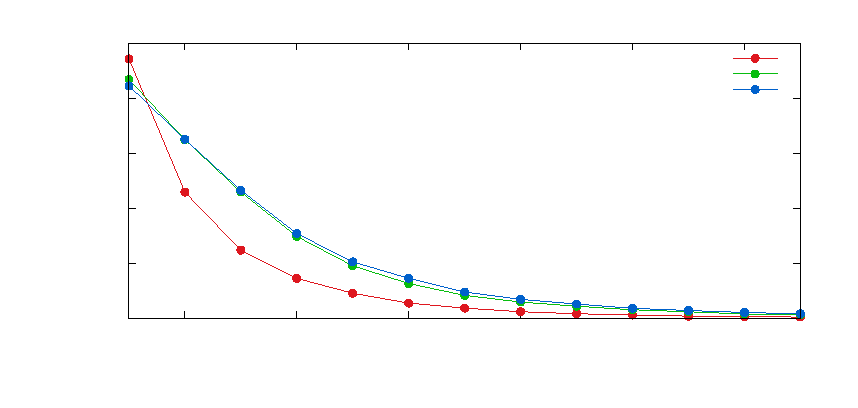
\includegraphics{../plots/arqtimeouts}}%
    \gplfronttext
  \end{picture}%
\endgroup

    \caption[Results for ARQ timeouts experiment]{long}
    \label{fig:resultsarqtimeouts}
\end{figure}

Figure \vref{fig:resultsarqtimeouts} shows the results for timeout values ranging from 3 to 15 cycles.

- Use sadias formula for RTB size estimation

We choose value of 12 because then for all NC variants, it is less than 1 ARQ per 100 source flits. Higher timeout would entail even less ARQs, but
increase latency and RTB sizes.

\subsection{Number Of Crypto Modules}
\begin{table}
    \centering
    \begin{tabulary}{\textwidth}{C|C|C|C|C|C|C|C|C}
        \pProtVar{} & \pNCMode{} & \pEncMods{} & \pAuthMods{} & \pARQLimit{} & \pARQTimeout{} & \pRStrat{} & \pNumAttackers{} & \pAttackProb{} \\\hline
        varying & varying & varying & varying & 1 & 12 & \gls{dor} & 8 & 0.2 \\
    \end{tabulary}
    \caption[Input parameters for number of crypto modules experiment]{long}
    \label{tab:setupnumcrypto}
\end{table}
- congestions in the queues in front of the crypto modules should be minimal
- less modules are better if possible because less chip area
- relatively high attack probabilities because more ARQs means more ver.+dec. retries at receivers, and network should be able to deal with that scenario
  "network needs to be equipped to deal with/handle periods of high traffic volumes"
- max. required enc. units: 4, because max. 2 flits can be drawn from the queues per cycle, so max. 4 flits active at the same time
- max. required auth. units: 12 (ind. auth), 10 (int. auth), 11 (gen. auth (2 flits = 11 cycles busy))
- criterion: max wait time needs to be 5 or less cycles

\begin{figure}
    \centering
    \begin{tabular}{ll}
        % GNUPLOT: LaTeX picture with Postscript
\begingroup
\newcommand{\ft}[0]{\footnotesize}\newcommand{\ty}[0]{\tiny}
  \makeatletter
  \providecommand\color[2][]{%
    \GenericError{(gnuplot) \space\space\space\@spaces}{%
      Package color not loaded in conjunction with
      terminal option `colourtext'%
    }{See the gnuplot documentation for explanation.%
    }{Either use 'blacktext' in gnuplot or load the package
      color.sty in LaTeX.}%
    \renewcommand\color[2][]{}%
  }%
  \providecommand\includegraphics[2][]{%
    \GenericError{(gnuplot) \space\space\space\@spaces}{%
      Package graphicx or graphics not loaded%
    }{See the gnuplot documentation for explanation.%
    }{The gnuplot epslatex terminal needs graphicx.sty or graphics.sty.}%
    \renewcommand\includegraphics[2][]{}%
  }%
  \providecommand\rotatebox[2]{#2}%
  \@ifundefined{ifGPcolor}{%
    \newif\ifGPcolor
    \GPcolortrue
  }{}%
  \@ifundefined{ifGPblacktext}{%
    \newif\ifGPblacktext
    \GPblacktextfalse
  }{}%
  % define a \g@addto@macro without @ in the name:
  \let\gplgaddtomacro\g@addto@macro
  % define empty templates for all commands taking text:
  \gdef\gplbacktext{}%
  \gdef\gplfronttext{}%
  \makeatother
  \ifGPblacktext
    % no textcolor at all
    \def\colorrgb#1{}%
    \def\colorgray#1{}%
  \else
    % gray or color?
    \ifGPcolor
      \def\colorrgb#1{\color[rgb]{#1}}%
      \def\colorgray#1{\color[gray]{#1}}%
      \expandafter\def\csname LTw\endcsname{\color{white}}%
      \expandafter\def\csname LTb\endcsname{\color{black}}%
      \expandafter\def\csname LTa\endcsname{\color{black}}%
      \expandafter\def\csname LT0\endcsname{\color[rgb]{1,0,0}}%
      \expandafter\def\csname LT1\endcsname{\color[rgb]{0,1,0}}%
      \expandafter\def\csname LT2\endcsname{\color[rgb]{0,0,1}}%
      \expandafter\def\csname LT3\endcsname{\color[rgb]{1,0,1}}%
      \expandafter\def\csname LT4\endcsname{\color[rgb]{0,1,1}}%
      \expandafter\def\csname LT5\endcsname{\color[rgb]{1,1,0}}%
      \expandafter\def\csname LT6\endcsname{\color[rgb]{0,0,0}}%
      \expandafter\def\csname LT7\endcsname{\color[rgb]{1,0.3,0}}%
      \expandafter\def\csname LT8\endcsname{\color[rgb]{0.5,0.5,0.5}}%
    \else
      % gray
      \def\colorrgb#1{\color{black}}%
      \def\colorgray#1{\color[gray]{#1}}%
      \expandafter\def\csname LTw\endcsname{\color{white}}%
      \expandafter\def\csname LTb\endcsname{\color{black}}%
      \expandafter\def\csname LTa\endcsname{\color{black}}%
      \expandafter\def\csname LT0\endcsname{\color{black}}%
      \expandafter\def\csname LT1\endcsname{\color{black}}%
      \expandafter\def\csname LT2\endcsname{\color{black}}%
      \expandafter\def\csname LT3\endcsname{\color{black}}%
      \expandafter\def\csname LT4\endcsname{\color{black}}%
      \expandafter\def\csname LT5\endcsname{\color{black}}%
      \expandafter\def\csname LT6\endcsname{\color{black}}%
      \expandafter\def\csname LT7\endcsname{\color{black}}%
      \expandafter\def\csname LT8\endcsname{\color{black}}%
    \fi
  \fi
    \setlength{\unitlength}{0.0500bp}%
    \ifx\gptboxheight\undefined%
      \newlength{\gptboxheight}%
      \newlength{\gptboxwidth}%
      \newsavebox{\gptboxtext}%
    \fi%
    \setlength{\fboxrule}{0.5pt}%
    \setlength{\fboxsep}{1pt}%
\begin{picture}(3600.00,3168.00)%
    \gplgaddtomacro\gplbacktext{%
      \csname LTb\endcsname%
      \put(858,660){\makebox(0,0)[r]{\strut{}\ft 1}}%
      \put(858,1782){\makebox(0,0)[r]{\strut{}\ft 10}}%
      \put(858,2903){\makebox(0,0)[r]{\strut{}\ft 100}}%
      \put(990,440){\makebox(0,0){\strut{}\ft 1}}%
      \put(1728,440){\makebox(0,0){\strut{}\ft 2}}%
      \put(2465,440){\makebox(0,0){\strut{}\ft 3}}%
      \put(3203,440){\makebox(0,0){\strut{}\ft 4}}%
    }%
    \gplgaddtomacro\gplfronttext{%
      \csname LTb\endcsname%
      \put(352,1781){\rotatebox{-270}{\makebox(0,0){\strut{}\ft Enqueued time in cycles}}}%
      \put(2096,154){\makebox(0,0){\strut{}\ft No. of encryption modules}}%
      \csname LTb\endcsname%
      \put(2468,2765){\makebox(0,0)[r]{\strut{}\ty IDA-UC max}}%
      \csname LTb\endcsname%
      \put(2468,2615){\makebox(0,0)[r]{\strut{}\ty avg}}%
      \csname LTb\endcsname%
      \put(2468,2465){\makebox(0,0)[r]{\strut{}\ty G2C3 max}}%
      \csname LTb\endcsname%
      \put(2468,2315){\makebox(0,0)[r]{\strut{}\ty avg}}%
      \csname LTb\endcsname%
      \put(2468,2165){\makebox(0,0)[r]{\strut{}\ty G2C4 max}}%
      \csname LTb\endcsname%
      \put(2468,2015){\makebox(0,0)[r]{\strut{}\ty avg}}%
    }%
    \gplbacktext
    \put(0,0){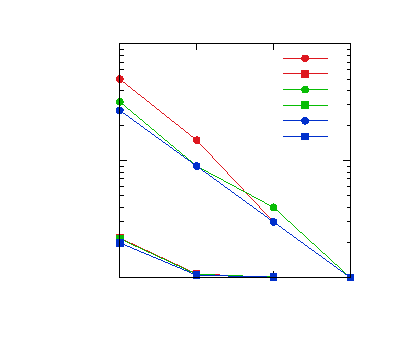
\includegraphics{../plots/encmodules-ida}}%
    \gplfronttext
  \end{picture}%
\endgroup
 & % GNUPLOT: LaTeX picture with Postscript
\begingroup
\newcommand{\ft}[0]{\footnotesize}\newcommand{\ty}[0]{\tiny}
  \makeatletter
  \providecommand\color[2][]{%
    \GenericError{(gnuplot) \space\space\space\@spaces}{%
      Package color not loaded in conjunction with
      terminal option `colourtext'%
    }{See the gnuplot documentation for explanation.%
    }{Either use 'blacktext' in gnuplot or load the package
      color.sty in LaTeX.}%
    \renewcommand\color[2][]{}%
  }%
  \providecommand\includegraphics[2][]{%
    \GenericError{(gnuplot) \space\space\space\@spaces}{%
      Package graphicx or graphics not loaded%
    }{See the gnuplot documentation for explanation.%
    }{The gnuplot epslatex terminal needs graphicx.sty or graphics.sty.}%
    \renewcommand\includegraphics[2][]{}%
  }%
  \providecommand\rotatebox[2]{#2}%
  \@ifundefined{ifGPcolor}{%
    \newif\ifGPcolor
    \GPcolortrue
  }{}%
  \@ifundefined{ifGPblacktext}{%
    \newif\ifGPblacktext
    \GPblacktextfalse
  }{}%
  % define a \g@addto@macro without @ in the name:
  \let\gplgaddtomacro\g@addto@macro
  % define empty templates for all commands taking text:
  \gdef\gplbacktext{}%
  \gdef\gplfronttext{}%
  \makeatother
  \ifGPblacktext
    % no textcolor at all
    \def\colorrgb#1{}%
    \def\colorgray#1{}%
  \else
    % gray or color?
    \ifGPcolor
      \def\colorrgb#1{\color[rgb]{#1}}%
      \def\colorgray#1{\color[gray]{#1}}%
      \expandafter\def\csname LTw\endcsname{\color{white}}%
      \expandafter\def\csname LTb\endcsname{\color{black}}%
      \expandafter\def\csname LTa\endcsname{\color{black}}%
      \expandafter\def\csname LT0\endcsname{\color[rgb]{1,0,0}}%
      \expandafter\def\csname LT1\endcsname{\color[rgb]{0,1,0}}%
      \expandafter\def\csname LT2\endcsname{\color[rgb]{0,0,1}}%
      \expandafter\def\csname LT3\endcsname{\color[rgb]{1,0,1}}%
      \expandafter\def\csname LT4\endcsname{\color[rgb]{0,1,1}}%
      \expandafter\def\csname LT5\endcsname{\color[rgb]{1,1,0}}%
      \expandafter\def\csname LT6\endcsname{\color[rgb]{0,0,0}}%
      \expandafter\def\csname LT7\endcsname{\color[rgb]{1,0.3,0}}%
      \expandafter\def\csname LT8\endcsname{\color[rgb]{0.5,0.5,0.5}}%
    \else
      % gray
      \def\colorrgb#1{\color{black}}%
      \def\colorgray#1{\color[gray]{#1}}%
      \expandafter\def\csname LTw\endcsname{\color{white}}%
      \expandafter\def\csname LTb\endcsname{\color{black}}%
      \expandafter\def\csname LTa\endcsname{\color{black}}%
      \expandafter\def\csname LT0\endcsname{\color{black}}%
      \expandafter\def\csname LT1\endcsname{\color{black}}%
      \expandafter\def\csname LT2\endcsname{\color{black}}%
      \expandafter\def\csname LT3\endcsname{\color{black}}%
      \expandafter\def\csname LT4\endcsname{\color{black}}%
      \expandafter\def\csname LT5\endcsname{\color{black}}%
      \expandafter\def\csname LT6\endcsname{\color{black}}%
      \expandafter\def\csname LT7\endcsname{\color{black}}%
      \expandafter\def\csname LT8\endcsname{\color{black}}%
    \fi
  \fi
    \setlength{\unitlength}{0.0500bp}%
    \ifx\gptboxheight\undefined%
      \newlength{\gptboxheight}%
      \newlength{\gptboxwidth}%
      \newsavebox{\gptboxtext}%
    \fi%
    \setlength{\fboxrule}{0.5pt}%
    \setlength{\fboxsep}{1pt}%
\begin{picture}(4464.00,3168.00)%
    \gplgaddtomacro\gplbacktext{%
      \csname LTb\endcsname%
      \put(858,660){\makebox(0,0)[r]{\strut{}\ft 1}}%
      \put(858,1782){\makebox(0,0)[r]{\strut{}\ft 10}}%
      \put(858,2903){\makebox(0,0)[r]{\strut{}\ft 100}}%
      \put(990,440){\makebox(0,0){\strut{}\ft 1}}%
      \put(1270,440){\makebox(0,0){\strut{}\ft 2}}%
      \put(1549,440){\makebox(0,0){\strut{}\ft 3}}%
      \put(1829,440){\makebox(0,0){\strut{}\ft 4}}%
      \put(2109,440){\makebox(0,0){\strut{}\ft 5}}%
      \put(2389,440){\makebox(0,0){\strut{}\ft 6}}%
      \put(2668,440){\makebox(0,0){\strut{}\ft 7}}%
      \put(2948,440){\makebox(0,0){\strut{}\ft 8}}%
      \put(3228,440){\makebox(0,0){\strut{}\ft 9}}%
      \put(3508,440){\makebox(0,0){\strut{}\ft 10}}%
      \put(3787,440){\makebox(0,0){\strut{}\ft 11}}%
      \put(4067,440){\makebox(0,0){\strut{}\ft 12}}%
    }%
    \gplgaddtomacro\gplfronttext{%
      \csname LTb\endcsname%
      \put(352,1781){\rotatebox{-270}{\makebox(0,0){\strut{}\ft Enqueued time in cycles}}}%
      \put(2528,154){\makebox(0,0){\strut{}\ft No. of authentication modules}}%
      \csname LTb\endcsname%
      \put(3332,2765){\makebox(0,0)[r]{\strut{}\ty IDA-UC max}}%
      \csname LTb\endcsname%
      \put(3332,2615){\makebox(0,0)[r]{\strut{}\ty avg}}%
      \csname LTb\endcsname%
      \put(3332,2465){\makebox(0,0)[r]{\strut{}\ty G2C3 max}}%
      \csname LTb\endcsname%
      \put(3332,2315){\makebox(0,0)[r]{\strut{}\ty avg}}%
      \csname LTb\endcsname%
      \put(3332,2165){\makebox(0,0)[r]{\strut{}\ty G2C4 max}}%
      \csname LTb\endcsname%
      \put(3332,2015){\makebox(0,0)[r]{\strut{}\ty avg}}%
    }%
    \gplbacktext
    \put(0,0){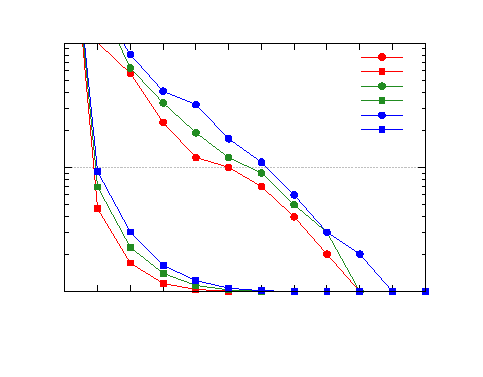
\includegraphics{../plots/authmodules-ida}}%
    \gplfronttext
  \end{picture}%
\endgroup
 \\
        % GNUPLOT: LaTeX picture with Postscript
\begingroup
\newcommand{\ft}[0]{\footnotesize}\newcommand{\ty}[0]{\tiny}
  \makeatletter
  \providecommand\color[2][]{%
    \GenericError{(gnuplot) \space\space\space\@spaces}{%
      Package color not loaded in conjunction with
      terminal option `colourtext'%
    }{See the gnuplot documentation for explanation.%
    }{Either use 'blacktext' in gnuplot or load the package
      color.sty in LaTeX.}%
    \renewcommand\color[2][]{}%
  }%
  \providecommand\includegraphics[2][]{%
    \GenericError{(gnuplot) \space\space\space\@spaces}{%
      Package graphicx or graphics not loaded%
    }{See the gnuplot documentation for explanation.%
    }{The gnuplot epslatex terminal needs graphicx.sty or graphics.sty.}%
    \renewcommand\includegraphics[2][]{}%
  }%
  \providecommand\rotatebox[2]{#2}%
  \@ifundefined{ifGPcolor}{%
    \newif\ifGPcolor
    \GPcolortrue
  }{}%
  \@ifundefined{ifGPblacktext}{%
    \newif\ifGPblacktext
    \GPblacktextfalse
  }{}%
  % define a \g@addto@macro without @ in the name:
  \let\gplgaddtomacro\g@addto@macro
  % define empty templates for all commands taking text:
  \gdef\gplbacktext{}%
  \gdef\gplfronttext{}%
  \makeatother
  \ifGPblacktext
    % no textcolor at all
    \def\colorrgb#1{}%
    \def\colorgray#1{}%
  \else
    % gray or color?
    \ifGPcolor
      \def\colorrgb#1{\color[rgb]{#1}}%
      \def\colorgray#1{\color[gray]{#1}}%
      \expandafter\def\csname LTw\endcsname{\color{white}}%
      \expandafter\def\csname LTb\endcsname{\color{black}}%
      \expandafter\def\csname LTa\endcsname{\color{black}}%
      \expandafter\def\csname LT0\endcsname{\color[rgb]{1,0,0}}%
      \expandafter\def\csname LT1\endcsname{\color[rgb]{0,1,0}}%
      \expandafter\def\csname LT2\endcsname{\color[rgb]{0,0,1}}%
      \expandafter\def\csname LT3\endcsname{\color[rgb]{1,0,1}}%
      \expandafter\def\csname LT4\endcsname{\color[rgb]{0,1,1}}%
      \expandafter\def\csname LT5\endcsname{\color[rgb]{1,1,0}}%
      \expandafter\def\csname LT6\endcsname{\color[rgb]{0,0,0}}%
      \expandafter\def\csname LT7\endcsname{\color[rgb]{1,0.3,0}}%
      \expandafter\def\csname LT8\endcsname{\color[rgb]{0.5,0.5,0.5}}%
    \else
      % gray
      \def\colorrgb#1{\color{black}}%
      \def\colorgray#1{\color[gray]{#1}}%
      \expandafter\def\csname LTw\endcsname{\color{white}}%
      \expandafter\def\csname LTb\endcsname{\color{black}}%
      \expandafter\def\csname LTa\endcsname{\color{black}}%
      \expandafter\def\csname LT0\endcsname{\color{black}}%
      \expandafter\def\csname LT1\endcsname{\color{black}}%
      \expandafter\def\csname LT2\endcsname{\color{black}}%
      \expandafter\def\csname LT3\endcsname{\color{black}}%
      \expandafter\def\csname LT4\endcsname{\color{black}}%
      \expandafter\def\csname LT5\endcsname{\color{black}}%
      \expandafter\def\csname LT6\endcsname{\color{black}}%
      \expandafter\def\csname LT7\endcsname{\color{black}}%
      \expandafter\def\csname LT8\endcsname{\color{black}}%
    \fi
  \fi
    \setlength{\unitlength}{0.0500bp}%
    \ifx\gptboxheight\undefined%
      \newlength{\gptboxheight}%
      \newlength{\gptboxwidth}%
      \newsavebox{\gptboxtext}%
    \fi%
    \setlength{\fboxrule}{0.5pt}%
    \setlength{\fboxsep}{1pt}%
\begin{picture}(3600.00,3168.00)%
    \gplgaddtomacro\gplbacktext{%
      \csname LTb\endcsname%
      \put(858,660){\makebox(0,0)[r]{\strut{}\ft 1}}%
      \put(858,1782){\makebox(0,0)[r]{\strut{}\ft 10}}%
      \put(858,2903){\makebox(0,0)[r]{\strut{}\ft 100}}%
      \put(990,440){\makebox(0,0){\strut{}\ft 1}}%
      \put(1728,440){\makebox(0,0){\strut{}\ft 2}}%
      \put(2465,440){\makebox(0,0){\strut{}\ft 3}}%
      \put(3203,440){\makebox(0,0){\strut{}\ft 4}}%
    }%
    \gplgaddtomacro\gplfronttext{%
      \csname LTb\endcsname%
      \put(352,1781){\rotatebox{-270}{\makebox(0,0){\strut{}\ft Enqueued time in cycles}}}%
      \put(2096,154){\makebox(0,0){\strut{}\ft No. of encryption modules}}%
      \csname LTb\endcsname%
      \put(2468,2765){\makebox(0,0)[r]{\strut{}\ty IWA-UC max}}%
      \csname LTb\endcsname%
      \put(2468,2615){\makebox(0,0)[r]{\strut{}\ty avg}}%
      \csname LTb\endcsname%
      \put(2468,2465){\makebox(0,0)[r]{\strut{}\ty G2C3 max}}%
      \csname LTb\endcsname%
      \put(2468,2315){\makebox(0,0)[r]{\strut{}\ty avg}}%
      \csname LTb\endcsname%
      \put(2468,2165){\makebox(0,0)[r]{\strut{}\ty G2C4 max}}%
      \csname LTb\endcsname%
      \put(2468,2015){\makebox(0,0)[r]{\strut{}\ty avg}}%
    }%
    \gplbacktext
    \put(0,0){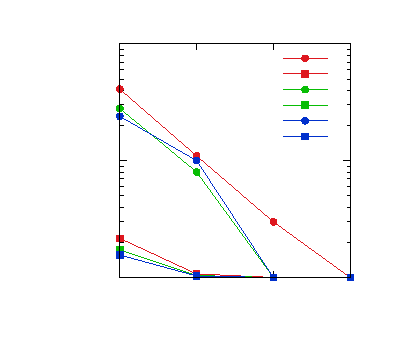
\includegraphics{../plots/encmodules-iwa}}%
    \gplfronttext
  \end{picture}%
\endgroup
 & % GNUPLOT: LaTeX picture with Postscript
\begingroup
\newcommand{\ft}[0]{\footnotesize}\newcommand{\ty}[0]{\tiny}
  \makeatletter
  \providecommand\color[2][]{%
    \GenericError{(gnuplot) \space\space\space\@spaces}{%
      Package color not loaded in conjunction with
      terminal option `colourtext'%
    }{See the gnuplot documentation for explanation.%
    }{Either use 'blacktext' in gnuplot or load the package
      color.sty in LaTeX.}%
    \renewcommand\color[2][]{}%
  }%
  \providecommand\includegraphics[2][]{%
    \GenericError{(gnuplot) \space\space\space\@spaces}{%
      Package graphicx or graphics not loaded%
    }{See the gnuplot documentation for explanation.%
    }{The gnuplot epslatex terminal needs graphicx.sty or graphics.sty.}%
    \renewcommand\includegraphics[2][]{}%
  }%
  \providecommand\rotatebox[2]{#2}%
  \@ifundefined{ifGPcolor}{%
    \newif\ifGPcolor
    \GPcolortrue
  }{}%
  \@ifundefined{ifGPblacktext}{%
    \newif\ifGPblacktext
    \GPblacktextfalse
  }{}%
  % define a \g@addto@macro without @ in the name:
  \let\gplgaddtomacro\g@addto@macro
  % define empty templates for all commands taking text:
  \gdef\gplbacktext{}%
  \gdef\gplfronttext{}%
  \makeatother
  \ifGPblacktext
    % no textcolor at all
    \def\colorrgb#1{}%
    \def\colorgray#1{}%
  \else
    % gray or color?
    \ifGPcolor
      \def\colorrgb#1{\color[rgb]{#1}}%
      \def\colorgray#1{\color[gray]{#1}}%
      \expandafter\def\csname LTw\endcsname{\color{white}}%
      \expandafter\def\csname LTb\endcsname{\color{black}}%
      \expandafter\def\csname LTa\endcsname{\color{black}}%
      \expandafter\def\csname LT0\endcsname{\color[rgb]{1,0,0}}%
      \expandafter\def\csname LT1\endcsname{\color[rgb]{0,1,0}}%
      \expandafter\def\csname LT2\endcsname{\color[rgb]{0,0,1}}%
      \expandafter\def\csname LT3\endcsname{\color[rgb]{1,0,1}}%
      \expandafter\def\csname LT4\endcsname{\color[rgb]{0,1,1}}%
      \expandafter\def\csname LT5\endcsname{\color[rgb]{1,1,0}}%
      \expandafter\def\csname LT6\endcsname{\color[rgb]{0,0,0}}%
      \expandafter\def\csname LT7\endcsname{\color[rgb]{1,0.3,0}}%
      \expandafter\def\csname LT8\endcsname{\color[rgb]{0.5,0.5,0.5}}%
    \else
      % gray
      \def\colorrgb#1{\color{black}}%
      \def\colorgray#1{\color[gray]{#1}}%
      \expandafter\def\csname LTw\endcsname{\color{white}}%
      \expandafter\def\csname LTb\endcsname{\color{black}}%
      \expandafter\def\csname LTa\endcsname{\color{black}}%
      \expandafter\def\csname LT0\endcsname{\color{black}}%
      \expandafter\def\csname LT1\endcsname{\color{black}}%
      \expandafter\def\csname LT2\endcsname{\color{black}}%
      \expandafter\def\csname LT3\endcsname{\color{black}}%
      \expandafter\def\csname LT4\endcsname{\color{black}}%
      \expandafter\def\csname LT5\endcsname{\color{black}}%
      \expandafter\def\csname LT6\endcsname{\color{black}}%
      \expandafter\def\csname LT7\endcsname{\color{black}}%
      \expandafter\def\csname LT8\endcsname{\color{black}}%
    \fi
  \fi
    \setlength{\unitlength}{0.0500bp}%
    \ifx\gptboxheight\undefined%
      \newlength{\gptboxheight}%
      \newlength{\gptboxwidth}%
      \newsavebox{\gptboxtext}%
    \fi%
    \setlength{\fboxrule}{0.5pt}%
    \setlength{\fboxsep}{1pt}%
\begin{picture}(4464.00,3168.00)%
    \gplgaddtomacro\gplbacktext{%
      \csname LTb\endcsname%
      \put(858,660){\makebox(0,0)[r]{\strut{}\ft 1}}%
      \put(858,1782){\makebox(0,0)[r]{\strut{}\ft 10}}%
      \put(858,2903){\makebox(0,0)[r]{\strut{}\ft 100}}%
      \put(990,440){\makebox(0,0){\strut{}\ft 1}}%
      \put(1270,440){\makebox(0,0){\strut{}\ft 2}}%
      \put(1549,440){\makebox(0,0){\strut{}\ft 3}}%
      \put(1829,440){\makebox(0,0){\strut{}\ft 4}}%
      \put(2109,440){\makebox(0,0){\strut{}\ft 5}}%
      \put(2389,440){\makebox(0,0){\strut{}\ft 6}}%
      \put(2668,440){\makebox(0,0){\strut{}\ft 7}}%
      \put(2948,440){\makebox(0,0){\strut{}\ft 8}}%
      \put(3228,440){\makebox(0,0){\strut{}\ft 9}}%
      \put(3508,440){\makebox(0,0){\strut{}\ft 10}}%
      \put(3787,440){\makebox(0,0){\strut{}\ft 11}}%
      \put(4067,440){\makebox(0,0){\strut{}\ft 12}}%
    }%
    \gplgaddtomacro\gplfronttext{%
      \csname LTb\endcsname%
      \put(352,1781){\rotatebox{-270}{\makebox(0,0){\strut{}\ft Enqueued time in cycles}}}%
      \put(2528,154){\makebox(0,0){\strut{}\ft No. of authentication modules}}%
      \csname LTb\endcsname%
      \put(3332,2765){\makebox(0,0)[r]{\strut{}\ty IWA-UC max}}%
      \csname LTb\endcsname%
      \put(3332,2615){\makebox(0,0)[r]{\strut{}\ty avg}}%
      \csname LTb\endcsname%
      \put(3332,2465){\makebox(0,0)[r]{\strut{}\ty G2C3 max}}%
      \csname LTb\endcsname%
      \put(3332,2315){\makebox(0,0)[r]{\strut{}\ty avg}}%
      \csname LTb\endcsname%
      \put(3332,2165){\makebox(0,0)[r]{\strut{}\ty G2C4 max}}%
      \csname LTb\endcsname%
      \put(3332,2015){\makebox(0,0)[r]{\strut{}\ty avg}}%
    }%
    \gplbacktext
    \put(0,0){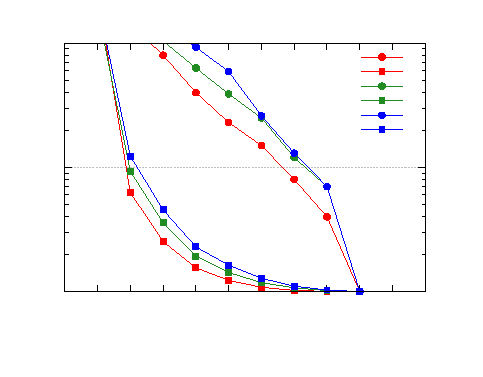
\includegraphics{../plots/authmodules-iwa}}%
    \gplfronttext
  \end{picture}%
\endgroup
 \\
        % GNUPLOT: LaTeX picture with Postscript
\begingroup
\newcommand{\ft}[0]{\footnotesize}\newcommand{\ty}[0]{\tiny}
  \makeatletter
  \providecommand\color[2][]{%
    \GenericError{(gnuplot) \space\space\space\@spaces}{%
      Package color not loaded in conjunction with
      terminal option `colourtext'%
    }{See the gnuplot documentation for explanation.%
    }{Either use 'blacktext' in gnuplot or load the package
      color.sty in LaTeX.}%
    \renewcommand\color[2][]{}%
  }%
  \providecommand\includegraphics[2][]{%
    \GenericError{(gnuplot) \space\space\space\@spaces}{%
      Package graphicx or graphics not loaded%
    }{See the gnuplot documentation for explanation.%
    }{The gnuplot epslatex terminal needs graphicx.sty or graphics.sty.}%
    \renewcommand\includegraphics[2][]{}%
  }%
  \providecommand\rotatebox[2]{#2}%
  \@ifundefined{ifGPcolor}{%
    \newif\ifGPcolor
    \GPcolortrue
  }{}%
  \@ifundefined{ifGPblacktext}{%
    \newif\ifGPblacktext
    \GPblacktextfalse
  }{}%
  % define a \g@addto@macro without @ in the name:
  \let\gplgaddtomacro\g@addto@macro
  % define empty templates for all commands taking text:
  \gdef\gplbacktext{}%
  \gdef\gplfronttext{}%
  \makeatother
  \ifGPblacktext
    % no textcolor at all
    \def\colorrgb#1{}%
    \def\colorgray#1{}%
  \else
    % gray or color?
    \ifGPcolor
      \def\colorrgb#1{\color[rgb]{#1}}%
      \def\colorgray#1{\color[gray]{#1}}%
      \expandafter\def\csname LTw\endcsname{\color{white}}%
      \expandafter\def\csname LTb\endcsname{\color{black}}%
      \expandafter\def\csname LTa\endcsname{\color{black}}%
      \expandafter\def\csname LT0\endcsname{\color[rgb]{1,0,0}}%
      \expandafter\def\csname LT1\endcsname{\color[rgb]{0,1,0}}%
      \expandafter\def\csname LT2\endcsname{\color[rgb]{0,0,1}}%
      \expandafter\def\csname LT3\endcsname{\color[rgb]{1,0,1}}%
      \expandafter\def\csname LT4\endcsname{\color[rgb]{0,1,1}}%
      \expandafter\def\csname LT5\endcsname{\color[rgb]{1,1,0}}%
      \expandafter\def\csname LT6\endcsname{\color[rgb]{0,0,0}}%
      \expandafter\def\csname LT7\endcsname{\color[rgb]{1,0.3,0}}%
      \expandafter\def\csname LT8\endcsname{\color[rgb]{0.5,0.5,0.5}}%
    \else
      % gray
      \def\colorrgb#1{\color{black}}%
      \def\colorgray#1{\color[gray]{#1}}%
      \expandafter\def\csname LTw\endcsname{\color{white}}%
      \expandafter\def\csname LTb\endcsname{\color{black}}%
      \expandafter\def\csname LTa\endcsname{\color{black}}%
      \expandafter\def\csname LT0\endcsname{\color{black}}%
      \expandafter\def\csname LT1\endcsname{\color{black}}%
      \expandafter\def\csname LT2\endcsname{\color{black}}%
      \expandafter\def\csname LT3\endcsname{\color{black}}%
      \expandafter\def\csname LT4\endcsname{\color{black}}%
      \expandafter\def\csname LT5\endcsname{\color{black}}%
      \expandafter\def\csname LT6\endcsname{\color{black}}%
      \expandafter\def\csname LT7\endcsname{\color{black}}%
      \expandafter\def\csname LT8\endcsname{\color{black}}%
    \fi
  \fi
    \setlength{\unitlength}{0.0500bp}%
    \ifx\gptboxheight\undefined%
      \newlength{\gptboxheight}%
      \newlength{\gptboxwidth}%
      \newsavebox{\gptboxtext}%
    \fi%
    \setlength{\fboxrule}{0.5pt}%
    \setlength{\fboxsep}{1pt}%
\begin{picture}(3600.00,3168.00)%
    \gplgaddtomacro\gplbacktext{%
      \csname LTb\endcsname%
      \put(858,660){\makebox(0,0)[r]{\strut{}\ft 1}}%
      \put(858,1782){\makebox(0,0)[r]{\strut{}\ft 10}}%
      \put(858,2903){\makebox(0,0)[r]{\strut{}\ft 100}}%
      \put(990,440){\makebox(0,0){\strut{}\ft 1}}%
      \put(1728,440){\makebox(0,0){\strut{}\ft 2}}%
      \put(2465,440){\makebox(0,0){\strut{}\ft 3}}%
      \put(3203,440){\makebox(0,0){\strut{}\ft 4}}%
    }%
    \gplgaddtomacro\gplfronttext{%
      \csname LTb\endcsname%
      \put(352,1781){\rotatebox{-270}{\makebox(0,0){\strut{}\ft Enqueued time in cycles}}}%
      \put(2096,154){\makebox(0,0){\strut{}\ft No. of encryption modules}}%
      \csname LTb\endcsname%
      \put(2468,2765){\makebox(0,0)[r]{\strut{}\ty FGA-G2C3 max}}%
      \csname LTb\endcsname%
      \put(2468,2615){\makebox(0,0)[r]{\strut{}\ty avg}}%
      \csname LTb\endcsname%
      \put(2468,2465){\makebox(0,0)[r]{\strut{}\ty G2C4 max}}%
      \csname LTb\endcsname%
      \put(2468,2315){\makebox(0,0)[r]{\strut{}\ty avg}}%
    }%
    \gplbacktext
    \put(0,0){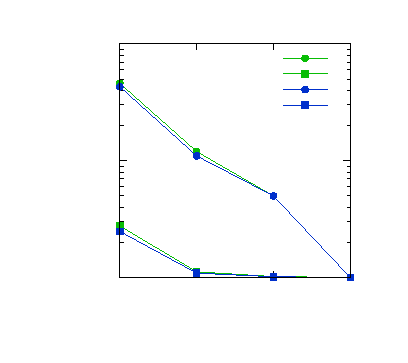
\includegraphics{../plots/encmodules-fga}}%
    \gplfronttext
  \end{picture}%
\endgroup
 & % GNUPLOT: LaTeX picture with Postscript
\begingroup
\newcommand{\ft}[0]{\footnotesize}\newcommand{\ty}[0]{\tiny}
  \makeatletter
  \providecommand\color[2][]{%
    \GenericError{(gnuplot) \space\space\space\@spaces}{%
      Package color not loaded in conjunction with
      terminal option `colourtext'%
    }{See the gnuplot documentation for explanation.%
    }{Either use 'blacktext' in gnuplot or load the package
      color.sty in LaTeX.}%
    \renewcommand\color[2][]{}%
  }%
  \providecommand\includegraphics[2][]{%
    \GenericError{(gnuplot) \space\space\space\@spaces}{%
      Package graphicx or graphics not loaded%
    }{See the gnuplot documentation for explanation.%
    }{The gnuplot epslatex terminal needs graphicx.sty or graphics.sty.}%
    \renewcommand\includegraphics[2][]{}%
  }%
  \providecommand\rotatebox[2]{#2}%
  \@ifundefined{ifGPcolor}{%
    \newif\ifGPcolor
    \GPcolortrue
  }{}%
  \@ifundefined{ifGPblacktext}{%
    \newif\ifGPblacktext
    \GPblacktextfalse
  }{}%
  % define a \g@addto@macro without @ in the name:
  \let\gplgaddtomacro\g@addto@macro
  % define empty templates for all commands taking text:
  \gdef\gplbacktext{}%
  \gdef\gplfronttext{}%
  \makeatother
  \ifGPblacktext
    % no textcolor at all
    \def\colorrgb#1{}%
    \def\colorgray#1{}%
  \else
    % gray or color?
    \ifGPcolor
      \def\colorrgb#1{\color[rgb]{#1}}%
      \def\colorgray#1{\color[gray]{#1}}%
      \expandafter\def\csname LTw\endcsname{\color{white}}%
      \expandafter\def\csname LTb\endcsname{\color{black}}%
      \expandafter\def\csname LTa\endcsname{\color{black}}%
      \expandafter\def\csname LT0\endcsname{\color[rgb]{1,0,0}}%
      \expandafter\def\csname LT1\endcsname{\color[rgb]{0,1,0}}%
      \expandafter\def\csname LT2\endcsname{\color[rgb]{0,0,1}}%
      \expandafter\def\csname LT3\endcsname{\color[rgb]{1,0,1}}%
      \expandafter\def\csname LT4\endcsname{\color[rgb]{0,1,1}}%
      \expandafter\def\csname LT5\endcsname{\color[rgb]{1,1,0}}%
      \expandafter\def\csname LT6\endcsname{\color[rgb]{0,0,0}}%
      \expandafter\def\csname LT7\endcsname{\color[rgb]{1,0.3,0}}%
      \expandafter\def\csname LT8\endcsname{\color[rgb]{0.5,0.5,0.5}}%
    \else
      % gray
      \def\colorrgb#1{\color{black}}%
      \def\colorgray#1{\color[gray]{#1}}%
      \expandafter\def\csname LTw\endcsname{\color{white}}%
      \expandafter\def\csname LTb\endcsname{\color{black}}%
      \expandafter\def\csname LTa\endcsname{\color{black}}%
      \expandafter\def\csname LT0\endcsname{\color{black}}%
      \expandafter\def\csname LT1\endcsname{\color{black}}%
      \expandafter\def\csname LT2\endcsname{\color{black}}%
      \expandafter\def\csname LT3\endcsname{\color{black}}%
      \expandafter\def\csname LT4\endcsname{\color{black}}%
      \expandafter\def\csname LT5\endcsname{\color{black}}%
      \expandafter\def\csname LT6\endcsname{\color{black}}%
      \expandafter\def\csname LT7\endcsname{\color{black}}%
      \expandafter\def\csname LT8\endcsname{\color{black}}%
    \fi
  \fi
    \setlength{\unitlength}{0.0500bp}%
    \ifx\gptboxheight\undefined%
      \newlength{\gptboxheight}%
      \newlength{\gptboxwidth}%
      \newsavebox{\gptboxtext}%
    \fi%
    \setlength{\fboxrule}{0.5pt}%
    \setlength{\fboxsep}{1pt}%
\begin{picture}(4320.00,3310.00)%
    \gplgaddtomacro\gplbacktext{%
      \csname LTb\endcsname%
      \put(330,660){\makebox(0,0)[r]{\strut{}\ft 1}}%
      \csname LTb\endcsname%
      \put(330,1853){\makebox(0,0)[r]{\strut{}\ft 10}}%
      \csname LTb\endcsname%
      \put(330,3045){\makebox(0,0)[r]{\strut{}\ft 100}}%
      \put(462,440){\makebox(0,0){\strut{}\ft 1}}%
      \put(777,440){\makebox(0,0){\strut{}\ft 2}}%
      \put(1091,440){\makebox(0,0){\strut{}\ft 3}}%
      \put(1406,440){\makebox(0,0){\strut{}\ft 4}}%
      \put(1721,440){\makebox(0,0){\strut{}\ft 5}}%
      \put(2035,440){\makebox(0,0){\strut{}\ft 6}}%
      \put(2350,440){\makebox(0,0){\strut{}\ft 7}}%
      \put(2664,440){\makebox(0,0){\strut{}\ft 8}}%
      \put(2979,440){\makebox(0,0){\strut{}\ft 9}}%
      \put(3294,440){\makebox(0,0){\strut{}\ft 10}}%
      \put(3608,440){\makebox(0,0){\strut{}\ft 11}}%
      \put(3923,440){\makebox(0,0){\strut{}\ft 12}}%
    }%
    \gplgaddtomacro\gplfronttext{%
      \csname LTb\endcsname%
      \put(-137,1852){\rotatebox{-270}{\makebox(0,0){\strut{}\ft Enqueued time in cycles}}}%
      \put(2192,154){\makebox(0,0){\strut{}\ft No. of authentication modules}}%
      \csname LTb\endcsname%
      \put(3224,2912){\makebox(0,0)[r]{\strut{}\ty FGA-G2C3 max}}%
      \csname LTb\endcsname%
      \put(3224,2772){\makebox(0,0)[r]{\strut{}\ty avg}}%
      \csname LTb\endcsname%
      \put(3224,2632){\makebox(0,0)[r]{\strut{}\ty G2C4 max}}%
      \csname LTb\endcsname%
      \put(3224,2492){\makebox(0,0)[r]{\strut{}\ty avg}}%
    }%
    \gplbacktext
    \put(0,0){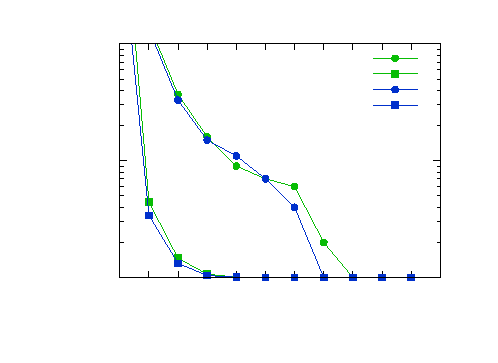
\includegraphics{../plots/authmodules-fga}}%
    \gplfronttext
  \end{picture}%
\endgroup

    \end{tabular}
    \caption[Results for number of crypto modules experiment]{The number of encryption modules (left column) and authentication modules (right column)
    is shown in relation to the maximum and average wait times of enqueued flits. Each row represents one protocol variant.}
    \label{fig:resultscryptomodules}
\end{figure}

\section{Experiments}
Record:
- acceptance rate (aka actual injection rate)
- information rate (source flits / total flits)
- residual error probability
- end-to-end latency
\subsection{Number of ARQs modified/dropped by routers}
\subsection{Routing strategies effects}
% Heatmap of router workload?

\iffalse
Experiment setup parameter tables:
- NC mode (UC, G2C3, G2C4)
- ...

ARQ Limit: 1, at most 2 because more ARQs allowed per transmission unit means larger retransmission buffers everywhere

\section{Statistics}
\begin{itemize}
    \item Injection/acceptance rate: [0, 1] (at processing element and at network interface)
    \item Queue lengths and buffer sizes
    \item Workload of crypto units
    \item Average/max flit waiting time at entry guard
    \item Average/max hop count
\end{itemize}

\section{Area Overhead}
\fi


    \chapter{Conclusion And Outlook}\label{ch:conclusion}
    In this thesis, a novel approach for securing the communications within a \gls{noc} against compromised routers with hardware trojans was presented
and evaluated. For this purpose, a protocol was designed that aims to ensure the protection goals of confidentiality and integrity. After examining
and assessing related work from this field of research, an in-depth explanation of said protocol was given. Several performance indicators were then
evaluated through extensive simulations with varying parameters. To conduct these experiment, a dedicated software was developed that facilitates
cycle-accurate analyses with detailed statistics for all facets of the protocol. Finally, the most suitable configuration was determined based on the
obtained results.

Future work:
\begin{itemize}
    \item Sequential IDs for uncoded and network coded → full transmission unit loss can be detected, ARQ issued
    \item Authenticated ARQs
    \item Different attacker models/smarter attackers
    \item If attacker model changes, i.e. attackers start to drop specific/whole generations,
        how does that influence the Routing/ARQ design? → ability to detect fully lost flits/gens via continuous IDs
    \item My idea of G3C4 with generation MAC as part of the G3? → it is feasible, would require experiments → G3C4 or G3C5? → refer to Yexin's
        experiments
    \item Authenticated encryption schemes in the NIs
    \item Local network coding, local encoding vectors
    \item Burst mode (w/ head and tail flits)
    \item TDM route selecting
    \item RNG for path selection in simulator → according to \cite{stefan11enhancingnocs}, non-static selection can be very expensive in area →
        explore static routes?
    \item Intelligent attackers → modify ARQs or send own ARQs → they are unauthenticated so DoS attack by maximizing retransmissions
    \item Usage of ECC (error correcting codes) to potentially reduce number of ARQs (at least for accidental bit flips)
    \item Security of the encryption → we kind of use ECB here which is not secure → e.g. a nonce is needed? or the flits need to be chained with some
        mode of operation like CBC or CTR → CBC requires no residual errors
    \item Mixing G2C3 and G2C4 -- e.g. once a network interface detects that it receives an unusually high amount of ARQs, indicating a very
        unreliable network, network coding could be \enquote{upgraded} from G2C3 to G2C4, so it is not statically one or the other
    \item Int. auth: adapt the scheme to compute MAC over the data part as well as just use the first 32 bit of the result as the "authcode". Saves a
        clock cycle because the cogwheel lookup function is omitted and input still fits into two blocks, but maybe security implications?
    \item Encryption (and encoding) of the address field → it may convey information useful to an attacker since the memory layout of the PEs is probably not random
        (→ ASLR?)
    \item Application of NC to ARQs (interwoven variant)
    \item Head-of-line blocking in routers → future work w/ virtual channels/TDM etc.
\end{itemize}


    % % % Glossary % % %
    \glsaddall % Print all glossary entries, not only the referenced ones (because some are only used in figures)
    \printglossaries
	
	% % % Bibliography % % %
	%\nocite{*} % Put all entries in the bibliography, not only those cited in the document
    \printbibliography[heading=bibintoc]
\end{document}
